%\documentclass[10pt,a4paper]{article}
\documentclass[12pt,a4paper]{article}
\usepackage{graphicx,units,amsmath}
\usepackage{subfigure}
\usepackage{float}
\usepackage[ngerman, english]{babel} 
%\usepackage[utf8]{inputenc}
\setcounter{secnumdepth}{4}
\usepackage[top=2cm, bottom=2.5cm, left=3cm, right=3cm]{geometry}

%-Eingabe der Metadaten des Titelblattes--------------------------

%-Daten des Autors / Authors Data---------------------------------

\newcommand{\dcauthorpre}{~} 
\newcommand{\dcauthorsurname}{Kullmann} 
\newcommand{\dcauthorname}{Richard} 
\newcommand{\dcauthoradd}{geboren am 17.07.1996 in Berlin-Pankow}

%-Titel und Untertitel / Title and subtitle-----------------------

\newcommand{\dctitle}{Giant Diffusion in two-dimensional Neuron Models} 
\newcommand{\dcsubtitle}{~}  
% Falls dcsubtitle NICHT verwendet werden soll, {\dcsubtitle}{~} eingeben.

%-Eingabe der Betreuuernahmen / Names of the consultants---------

\newcommand{\dcconsulta}{~} 
\newcommand{\dcconsultb}{~} 
\newcommand{\dcconsultc}{~} 

%-Eingabe der Gutachternamen / Names of the approvals-------------

\newcommand{\dcapprovala}{Prof. Dr. Benjamin Lindner} 
\newcommand{\dcapprovalb}{Prof. Dr. Igor Sokolov} 
\newcommand{\dcapprovalc}{~} 

%-Information zur Universitaet------------------------------------

\newcommand{\dcdegree}{Master of Science\\(M. Sc.)} 
\newcommand{\dcsubject}{Physik} 
\newcommand{\dcfaculty}{Mathematisch-Naturwissenschaftlichen Fakult\"at I}
\newcommand{\dcinstitute}{Institut f\"ur Physik}
\newcommand{\dcuniversity}{Humboldt-Universit\"at zu Berlin}
\newcommand{\dcdean}{Prof. Dr. sc. Heinz  M\"uller}
\newcommand{\dcpresident}{Prof. Dr. Dr. h.c. Wilhelm Schulz}

%-Pruefungsdaten: eingereicht und mdl. Pruefung-------------------
%-data of submission and oral exam--------------------------------

\newcommand{\dcdatesubmitted}{5. Juni 2020} %auch wenn nicht auf dem 
%Titelblatt, bitte erf�llen!
\newcommand{\dcdateexam}{2. Juli 1999} 


% Folgende Zeile bitte nicht aendern!
\newcommand{\dckeywordsde}{\vfill \raggedright {\textbf{Schlagw\"orter:}}\\ \dckeydea, \dckeydeb, \dckeydec, \dckeyded \\}

%-englische Schlagwoerter / english keywords----------------------

\newcommand{\dckeyena}{Giant Diffusion}
\newcommand{\dckeyenb}{Two-Dimensional Neuron Models}
\newcommand{\dckeyenc}{Bistability}
\newcommand{\dckeyend}{Signal-to-Noise Ratio}

% Folgende Zeile bitte nicht aendern!
\newcommand{\dckeywordsen}{\vfill \raggedright {\textbf{Keywords:}}\\ \dckeyena, \dckeyenb, \dckeyenc, \dckeyend \\}

\newcommand{\dcpdfsubject}{Dissertation}  
\graphicspath{{images/}}
\begin{document}


%\title{Bachelorarbeit}
%\author{Richard Kullmann}
%\date{02.06.2017}

%----------Generierung der Titelseite-----bitte nicht ver�ndern!--------------------


\author{von \\ \dcauthorpre\ \dcauthorname\ \dcauthorsurname\ \\ \dcauthoradd}

%----------
\title{ \vspace{-2cm}\dctitle \\ 
\vspace{0.5cm}
\large{\dcsubtitle} \\ 
\vspace{0.5cm} {\Large{MASTERARBEIT}}\\ 
\vspace{0.5cm} \large{zur Erlangung des akademischen Grades \\ 
\dcdegree\\ im Fach \dcsubject \\\vspace{0.5cm}

\includegraphics[width=6cm]{husiegel}\\ 
\vspace{0.5cm} eingereicht an der \\ 
\dcfaculty \\ 
\dcinstitute\\
\dcuniversity \\}}
%-----------------
\date{\vspace{2.5cm}
%\raggedright{
%Pr\"asident der Humboldt-Universit\"at zu Berlin:\\
%\dcpresident \vspace{-0.3cm}
%}\vspace{0.5cm}\\
%
%\raggedright{
%Dekan der \dcfaculty:\\
%\dcdean \vspace{-0.3cm}
%}\vspace{0.5cm}\\
%
% auskommentiert weil nicht standard
\raggedright{
Gutachter:
\begin{enumerate} 
\item{\it\dcapprovala} \vspace{-0.3cm}
\item{\it\dcapprovalb} \vspace{-0.3cm}
%\item{\it\dcapprovalc} \vspace{-0.3cm}
\end{enumerate}} \vspace{0.5cm}
%\raggedright{
%Betreuung:
%\begin{enumerate} 
%\item{\it\dcconsulta} \vspace{-0.2cm}
%\item{\it\dcconsultb} \vspace{-0.2cm}
%\end{enumerate}} \vspace{0.5cm}
%-----------------
\raggedright{
\begin{tabular}{lll}
eingereicht am: &  &\it\dcdatesubmitted\\ % wenn nicht in der Pr�fungsordnung, die Zeile bitte auskommentieren
%Tag der m\"undlichen Pr\"ufung: & & \dcdateexam
\end{tabular}}\\ 
}
%------------------------------------- 

\maketitle

\thispagestyle{empty}
%\setcounter{page}{2}
\newpage
%-englische-Zusammenfassung---------------------------------------

%\selectlanguage{english}

%\begin{abstract}
%\setcounter{page}{2} % Nach Bedarf anpassen!
%Here is the english abstract.\\
% hier werden die englische Schlagw�rter aus Metadaten �bernommen
%\dckeywordsen				
%\end{abstract}

%-deutsche Zusammenfassung----------------------------------------

%\selectlanguage{german}

\begin{abstract}
\setcounter{page}{2} % Nach Bedarf anpassen!
The emerging field of magnetometry based on NV centers opens a variety of new experimental perspectives, including the imaging of single nuclear spins on the nanoscale. However, in order to achieve exceptionally long NV electron spin coherence times and high sensitivities, the NV spin needs to be decoupled from unwanted interactions with the environment. This can be accomplished with dynamical decoupling sequences.
\\
During the work for this thesis, multiple dynamical decoupling protocols were implemented and tested on NV centers in bulk diamond and nanodiamond. 
\\
The theoretical part covers general NV properties before treating the behaviour of a free electron spin and finally applying this on the NV center. Then, the effect of different decoupling protocols are discussed. After that, the structure and concept of the setup will be explained. In the final part, the measurements will be presented. The execution of the decoupling sequences will be demonstrated and the data will be used to extract the spectral density function of the environment.
\\
It was shown that all implemented dynamical decoupling sequences could enhance the coherence time. It was demonstrated that CPMG outperforms the other sequences on the given setup, achieving an improvement of up to a factor of 200 in the bulk diamond and 50 in nanodiamond. Finally, the examination of the spectral density functions of the spin bath gave a deeper insight in its coupling strength to the NV and its internal dynamics.\\
In the future, the limitations of the sequences will be further explored and other decoupling protocols will be tested. In addition to that, a better time and phase control has to be accomplished. These efforts will eventually lead to sensitivities high enough to detect small spin ensembles and even single molecular spins.
% hier werden die deutsche Schlagw�rter aus Metadaten �bernommen
%\dckeywordsde
\end{abstract}
\thispagestyle{empty}

\tableofcontents
\thispagestyle{empty}
\newpage
\pagenumbering{arabic}

\section{Introduction}
By the end of the 20th century, the possibility of creating and manipulating single quantum systems has given rise to a manifold of new scientific and technological developments. Among these, quantum magnetic field imaging has attracted a lot of attention due to the unprecedented spatial and quantitative resolution that has been achieved through it. Several physical systems have been successfully exploited in this sense, ranging from Superconductive Quantum Interference Devices (SQUID)\cite{squid} to atomic vapor cells\cite{avc}. Solid state single defect centers have attracted a strong interest due to their capability of being operated at room temperature and within complex environments such as biological samples. In this case, the working principle is based on having a controlled interaction between a manipulable solid state spin and the magnetic target. Its successful implementation requires a stable and controllable quantum system which can be easily prepared and read out. Recently, it has been shown that the Nitrogen-Vacancy (NV) defect center in diamond satisfies these conditions and is a promising candidate for the realization of this technique since it possesses a stable electronic spin that can be manipulated and read out even at room temperature conditions\cite{nvref}. In order to achieve a high sensitivity, it's crucial to decouple the spin from interactions with the environment. This can be accomplished through dynamical decoupling techniques.\\
The goal of this thesis was the implementation of different decoupling techniques on single NV centers in nanodiamond and ensembles of NVs in a single crystal Bulk diamond, respectively.

\section{Theory}
\subsection{Diamond}
The nitrogen vacancy center is a point defect that consists of a substitutional nitrogen atom and an adjacent carbon vacancy in the diamond lattice. The latter is formed by pairs of carbon atoms arranged in a fcc structure. The equilibrium distance between the biatomic bases is $R_0=\unit[3,57]{\r{A}}$. Furthermore, diamond is an electric insulator with a bandgap of $E_g=\unit[5,5]{eV}$\cite{gmf}.
\subsubsection{Type classification of diamond}
Naturally available diamonds show a wide range of lattice impurities and defects. So, the type classification system is based on the occurrence of the two most common impurities: boron or nitrogen. Two major distinctions are made: type I diamonds contain enough N atoms to be detected by IR absorption spectroscopy while the concentration of N in type II diamonds is not high enough to be measured\cite{pod}. Type I diamonds are further divided into the types Ia and Ib. In Ia diamond, nitrogen occurs in small aggregates with a concentration up to 3000 ppm, whereas type Ib contains isolated single nitrogen atoms at concentrations up to 500 ppm\cite{mspd}. 
Type II diamonds are also divided into two more types: IIa and IIb. IIa diamonds contain fewer than a few ppm nitrogen or boron impurities and IIb diamonds are characterized by boron impurities which are considered to be isolated substitutional atoms and occur in concentrations below 500 ppm\cite{pod}\cite{cod}\cite{darm}\cite{opdadh}.
\subsubsection{Diamond crystals and nanoparticles}
Diamond is available in several forms, including single  and poly-cristalline gem stones or chips, micro-sized particles and nanocrystals as well. In this work, two different kind of samples have been examined: a single-crystal bulk diamond chip and a  batch of nanodiamonds. Bulk diamond can be found in nature or synthethized via High Pressure High Temperature (HPHT) or Chemical Vapour Deposition (CVD) growth\cite{dgcvd}\cite{hpht}. nanodiamonds are instead generally produced via detonation, but synthesis methods also include ion bombarding and Laser treatment, CVD as well as ultrasonic, hydrothermal and electrochemical techniques\cite{st}\cite{nd}. Shallow NVs in bulk and nanodiamond  have properties influenced not only by the diamond lattice itself but also by surface effects, whereas deeply buried nitrogen vacancies in the bulk show generally longer coherence times and interact mainly with the surrounding lattice atoms.
\subsection{Physical properties of the NV defect center}
A nitrogen-vacancy-center consists of a nitrogen atom (N) replacing a carbon atom, which is located next to a vacancy (V) in the diamond crystal lattice. There have been found two different types of NV-centers so far: the neutral NV$^0$ and the negatively charged NV$^-$ where an additional electron is captured from the diamond lattice. Due to its well-known and useful optical properties, only the latter has been the subject of interest in this work. Therefore it will just be referred to as NV in the following. \\
\begin{figure}[H]
    \subfigure[]{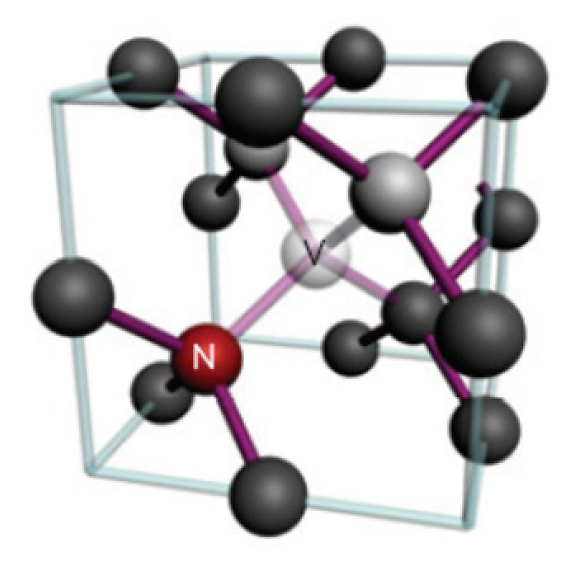
\includegraphics[width=0.45\textwidth]{nv.png}} 
    \subfigure[]{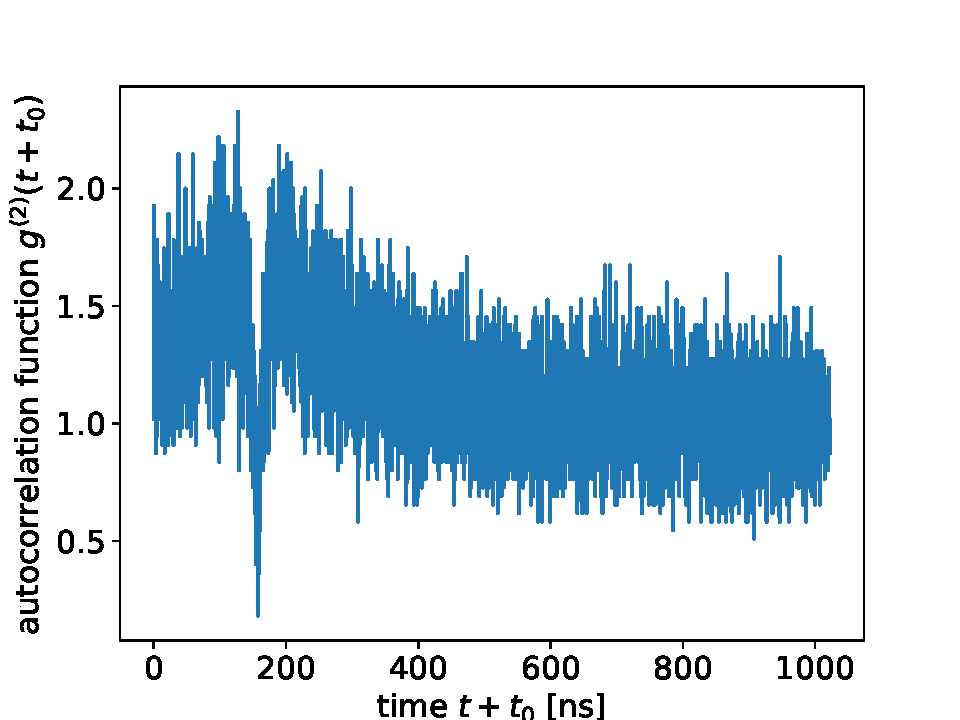
\includegraphics[width=0.65\textwidth]{autoc4.pdf}} 
    \caption{Figure (a) shows the structure of an NV-center in the diamond lattice (taken from \cite{repprog}), on the right one can see an autocorrelation measurement on an NV-center. A delay was added so that the minimum was not at $t=0$ and could be easily recognized.}
\label{acm} 
\end{figure}
The NV center is an atom - like system having its ground and first excited electronic states within the diamond bandgap. It is optically stable, showing neither photoblinking nor photobleaching, and has a long electron spin coherence time even at room temperature. Furthermore, its electron spin state can be optically initialized and read out as it emits in the visible light range where high efficiency detectors are available. Another striking property is its single photon fluorescence emission which makes it useful in quantum computation and quantum cryptography\cite{qr}\cite{qc} and allows us to identify single NVs using photon autocorrelation measurements as depicted in figure \ref{acm}.\\
A three-level system can be used to describe the optical properties of the NV center. By combining the experimental evidence with linear combination of atomic orbitals (LCAO) theory\cite{lar}, an optical ground state $^3A$ having three spin sublevels is identified. The $m_s=0$ and $m_s= \pm 1$ sublevels are separated by $D=2.87$ GHz when no magnetic field is applied. Two spin conserving optical dipole transitions connect the ground state with the first optical excited state $^3E$. After being excited, the nitrogen vacancy can radiatively relax back to the $^3A$ level, producing broadband photoluminescence (PL) with a zero-phonon line at 637 nm. Another possible de-excitation path is the non radiative relaxation, that occours via intersystem crossing (ISC) to a singlet state $^1A$. The ISCs to the singlet state are strongly spin selective as they have a higher probability to involve transitions from the $m_s=\pm 1$ sublevels than from $m_s=0$. Furthermore, from the $^1A$ state, the decay rate to the $m_s=0$ sublevel is much higher than to $m_s=\pm 1$. These spin-selective relaxation processes form the basis for the optical detection of magnetic resonance (ODMR). A change of the spin state will lead to a different fluorescence intensity from the defect center, with the highest intensity being detected for the pure $m_s=0$ state. Additionally, optical pumping allows a high degree of $m_s=0$ spin polarization. \\
\begin{figure}[H]
\centering
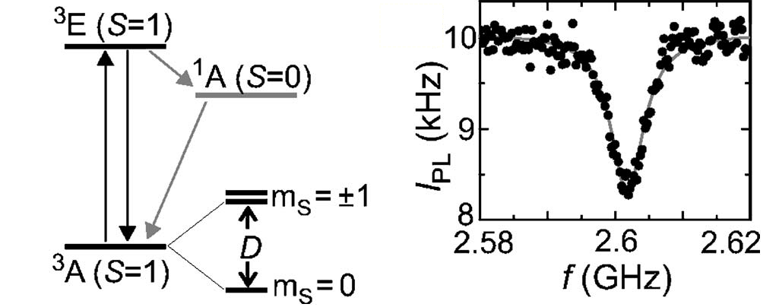
\includegraphics[scale=0.4]{energy_levels.png} 
\caption{General properties of NVs: on the left one can see the three-level structure of the NV, the right image shows an ESR measurement on an NV placed in a static magnetic field that splits the $m_s=\pm1$ sublevels. Thus, the resonant frequency lies below 2.87 GHz. This picture was taken from \cite{nv1}.}
\label{el}
\end{figure}
Similarly to the principle of nuclear magnetic resonance, the application of a microwave pulse can initiate transitions between the $m_s=0$ and $m_s=\pm1$ sublevels, if the resonance condition is fulfilled, $\nu_{MW}=D$. Consequently, if a resonant magnetic field is applied to an optically pumped NV, one observes a drop in PL intensity, as the $m_s=0$ population decreases. Furthermore, when the NV is placed in a static magnetic field, the Zeeman effect lifts the $m_s=\pm 1$ degeneracy, resulting in two resonance lines in the ESR spectrum. This allows the use of NV centers as magnetic sensors on an atomic scale\cite{repprog}\cite{nv1}. \\
\subsection{Second order correlation function}\label{g2}
NVs are single photon sources. This means, that a single NV can only emit one photon at a time. First, one excites the NV center and drives an optical dipole transition to the excited state. Then the excited state relaxes radiatively to the ground state or non radiatively through the metastable $^1A$ state. Therefore, no more than one photon is emitted at a time. As a result, the intensity correlation function of an NV shows a characteristic behaviour and can be used to identify single NVs. \\
The intensity correlation function of the light can be found by making two intensity measurements with a fixed time delay $\tau$ and averaging the product of the readings. The normalized form of this function is called \textit{degree of second-order temporal coherence} and is defined as:
\begin{equation}
g^{(2)}(\tau)=\frac{\langle\bar{I}(t)\bar{I}(t+\tau)\rangle}{\bar{I}^2}=\frac{\langle E^*(t)E^*(t+\tau)E(t+\tau)E(t)\rangle}{\langle E^*(t)E(t)\rangle^2}
\end{equation}
where $\bar{I}$ is the averaged intensity\cite{qtl}. For a single-mode light field, the coherence function at $\tau =0$ can be expressed in terms of the \textit{destruction} and \textit{creation operators}:
\begin{equation}
g^{(2)}(0)=\frac{\langle \hat{a}^\dag\hat{a}^\dag\hat{a}\hat{a}\rangle}{\langle\hat{a}^\dag\hat{a}\rangle ^2}
\end{equation}

Considering that $[\hat{a},\hat{a}^\dag]=1$ and $\hat{n}=\hat{a}^\dag\hat{a}$, one gets:
\begin{equation}
g^{(2)}(0)=\frac{\langle n^2\rangle -\langle n\rangle}{\langle n\rangle ^2}
\end{equation}
The fluorescence of single photon sources can be described with a Fock state, for which $\langle n\rangle =n$ and $\langle n^2\rangle =n^2$, so that follows:
\begin{equation}
g^{(2)}(0)=1-\frac{1}{n}
\end{equation}
In particular for a single NV center it is $n=1$ and thereby $g^{(2)}(0)=0$.
\subsection{The Electron Spin}
In order to model the NV center spin dynamics, we start by describing the behaviour of a simpler system, which is a single spin qubit. In this case the Bloch notation turns out to be practical.\\
An arbitrary state of a two-level system can be written as:
\begin{equation}\label{ab}
|\psi\rangle =\alpha |1\rangle +\beta |0\rangle =\alpha \left(\begin{matrix}
1\\0
\end{matrix}\right) + \beta \left(\begin{matrix}
0\\1
\end{matrix}\right)=\left(\begin{matrix}
\alpha \\\beta
\end{matrix}\right)
\end{equation}
where $|1\rangle$ and $|0\rangle$ are two orthogonal vectors representing the pure states.
Taking into account the normalization condition $\langle\psi |\psi\rangle=|\alpha |^2+|\beta |^2=1$, and neglecting a global phase without physical significance, one can rewrite this as:
\begin{equation}\label{bloch}
|\psi \rangle =\cos\frac{\theta}{2}|1\rangle +e^{i\phi}\sin\frac{\theta}{2}|0\rangle
\end{equation}
by introducing the angles $\theta$ and $\phi$. Thus, an arbitrary state can be represented as a unitary vector on the Bloch sphere, a 3-D unit sphere.\\
This notation will be used in the following to describe spin manipulations.
\subsection{Rabi Oscillations}\label{rabi}
By placing the single spin in a static magnetic field aligned along the z axis of the reference system, the degenerate energy levels split up due to the Zeeman effect. The Hamiltonian of this interaction is:
\begin{equation}
\hat{H}_Z=-\hat{\mu}_S\hat{B}
\end{equation}
where $\hat{\mu}_S$ is the spin magnetic moment and $\hat{B}$ the magnetic field. Using $\hat{\mu}_S=\gamma_S\hat{S}$ with $\gamma$ being the gyromagnetic ratio, $H_Z$ can be written as:
\begin{equation}\label{hz}
\hat{H}_Z=-\gamma_S\hat{S}\hat{B}=-\gamma_S\hat{S}_zB_z=-\frac{\gamma_S\hbar B_z}{2}\hat{\sigma}_z=\frac{\hbar}{2}\omega_B\hat{\sigma}_z
\end{equation}
where we introduced the Larmor frequency $\omega_{B}$ and the Pauli matrix $\sigma_z$. By adding an oscillatory magnetic field of the form \cite{bel}:
\begin{equation}
\hat{B}=B_1(\hat{x}\cos\omega t-\hat{y}\sin\omega t)
\end{equation}
the interaction Hamiltonian reads:
\begin{equation}
\hat{H}_B=-\hat{\mu}\hat{B}=-\gamma\hat{B}\hat{S}=-\gamma B_1(\hat{S}_x\cos\omega t-\hat{S}_y\sin\omega t)
\end{equation}
where $\hat{\mu}$ and $\gamma$ are the magnetic moment and gyromagnetic ratio of the system, and $\hat{S}$ is the spin operator. 
Expressing the spin components through the Pauli matrices using $\hat{S}_i=\frac{\hbar}{2}\hat{\sigma}_i$, we finally obtain:
\begin{equation}
\hat{H}_B=-\gamma\frac{\hbar}{2}\left(B_1(\cos\omega t\hat{\sigma}_x-\sin\omega t\hat{\sigma}_y)\right)
\end{equation}
This yields the total Hamiltonian:
\begin{equation}
\hat{H}=\hat{H}_Z+\hat{H}_B=\left(\begin{matrix}
\frac{\hbar\omega_{B}}{2}&-\gamma\frac{\hbar}{2}B_1(\cos\omega t+i\sin\omega t)\\
-\gamma\frac{\hbar}{2}B_1(\cos\omega t-i\sin\omega t)&-\frac{\hbar\omega_ {B}}{2}
\end{matrix}\right)
\end{equation}
For simplicity, we introduce the Larmor frequency $\omega_1 =\gamma B_1$ and express the oscillating terms using the complex exponential function:
\begin{equation}
\hat{H}=\frac{\hbar}{2}\left(\begin{matrix}
\omega_{B}&-\omega_1e^{i\omega t}\\
-\omega_1e^{-i\omega t}&-\omega_ {B}
\end{matrix}\right)
\end{equation}
For $\omega_{B}\gg\omega_1$, the eigenstates of the Hamiltonian remain basically unchanged. This allows us to use perturbation theory for the further investigation of the behaviour of the system. \\
The coefficients from equation (\ref{ab}) are now time-dependent and have to fulfil the following relations\cite{qmg}:
\begin{equation}
\dot{\alpha}=-\frac{i}{\hbar}H_{01}'e^{-i\omega_{10}t}\beta,\qquad\dot{\beta}=-\frac{i}{\hbar}H_{10}'e^{i\omega_{10}t}\alpha
\end{equation}
if the diagonal elements of the perturbation Hamiltonian $H'$ are zero. This translates into a second order differential equation:
\begin{equation}
\ddot{\alpha}=-\frac{1}{\hbar^2}H_{01}'H_{10}'\alpha-i\omega_{10}\dot{\alpha}+\frac{1}{H_{01}'}\frac{\partial H_{01}'}{\partial t}\dot{\alpha}
\end{equation}
With $H_{01}'=H_{10}'^*=-\frac{\hbar\omega_1}{2}e^{i\omega t}$, we get
\begin{equation}
\ddot{\alpha}-i(\omega-\omega_{10})\dot{\alpha}+\frac{\omega_1^2}{4}\alpha=0
\end{equation}
Using the ansatz $\alpha=e^{\lambda t}$, we find:
\begin{equation}
\lambda_{\pm}=\frac{i}{2}\left(\omega-\omega_{10}\pm\sqrt{(\omega-\omega_{10})^2+\omega_1^2}\right)
\end{equation}
This gives us the general solution:
\begin{equation}
\alpha(t)=c_1e^{\lambda_+t}+c_2e^{\lambda_-t}
\end{equation}
Let the system be in state $|1\rangle$ at $t=0$, providing the initial conditions $\alpha(0)=1$ and $\beta(0)=0$ and thereby giving the final result for $\alpha(t)$:
%\begin{align}
%\alpha(0)=1=c_1+c_2\Leftrightarrow c_1=1-c_2\\
%\beta(0)=0\Leftrightarrow\dot{\alpha}(0)=(1-c_2)\lambda_++c_2\lambda_-=0\\
%\Rightarrow c_1=-\frac{\lambda_-}{\lambda_+-\lambda_-},\qquad c_2=\frac{\lambda_+}{\lambda_+-\lambda_-}
%\end{align}  
%So, the final result for $\alpha(t)$ is:
\begin{equation}
\alpha(t)=-\frac{\lambda_-}{\lambda_+-\lambda_-}e^{\lambda_+t}+\frac{\lambda_+}{\lambda_+-\lambda_-}e^{\lambda_-t}
\end{equation}
Now, the probability of the system going to state $|0\rangle$ can be found using the normalization condition:
\begin{align}
P_{1\rightarrow 0}(t)=|\beta(t)|^2=1-|\alpha(t)|^2
%=1-\frac{\lambda_+^2+\lambda_-^2}{(\lambda_+-\lambda_-)^2}+\frac{2\lambda_+\lambda_-}{(\lambda_+-%\lambda_-)^2}\cos((\lambda_+-\lambda_-)t)\\
%=\frac{-2\lambda_+\lambda_-}{(\lambda_+-\lambda_-)^2}(1-\cos((\lambda_+-\lambda_-)t))
=\frac{-4\lambda_+\lambda_-}{(\lambda_+-\lambda_-)^2}\sin^2\left(\frac{i(\lambda_+-\lambda_-)t}{2}\right)
\end{align}
Substituting the values of $\lambda_\pm$, we find:
\begin{equation}
P_{1\rightarrow 0}(t)=\frac{\omega_1^2}{(\omega-\omega_{10})^2+\omega_1^2}\sin^2\left(\frac{\sqrt{(\omega-\omega_{10})^2+\omega_1^2}}{2}t\right)
\end{equation}
This result is known as Rabi's formula. \\
When the frequency of the oscillating field $B_1$ equals the energy separation between the two states, $\omega_{10}=\omega_{01}=\omega$, the resonant condition is satisfied and the transition probability is simplified as:
\begin{equation}
P_{1\rightarrow 0}(t)=\sin^2\left(\frac{\omega_1 t}{2}\right)
\end{equation}
So for a magnetic pulse of length $\omega_1 t=\pi \Leftrightarrow t=\nicefrac{\pi}{\omega_1}$ the system undergoes a complete transition from the ground state to the excited state. This corresponds to a rotation on the Bloch sphere by an angle of $\pi$ and is hence called a $\pi$ pulse. Applying a pulse of only half this length creates a coherent superposition of both states of equal weight, comparable to a rotation by the angle $\nicefrac{\pi}{2}$ and therefore called $\nicefrac{\pi}{2}$ pulse.

\subsection{Density matrix}\label{DM}
%C. Lü et al.,Spin relaxation time, spin dephasing time and ensemble spin dephasing time
%in n-type GaAs quantum wells,Physics Letters A 365, 2007.
%Claude Cohen-Tannoudji etal., Quantum mechanics. Wiley, 1977.
Until now any interaction process between the two level system and the external environment has been neglected. In order to take these phenomena into account, we may take advantage of the density matrix formalism. Here, a density operator can be defined as:
\begin{equation}
\hat{\rho}=|\psi(t)\rangle\langle\psi(t)|
\end{equation}
Keeping the notation from equation (\ref{ab}), this gives for a two-level system:
\begin{equation}
\hat{\rho}=\left(\begin{matrix}
|\alpha|^2&\alpha\beta^*\\\beta\alpha^*&|\beta|^2
\end{matrix}\right)
\end{equation}
The diagonal elements are equivalent to the probabilities of finding the system in its eigenstates $|0\rangle$ or $|1\rangle$. Therefore, they are called  \textit{populations} and it is $\rho_{11}+\rho_{22}=1$. The off-diagonal elements are called \textit{coherences}\cite{nmr}.\\
From the Schr\"odinger equation we obtain\cite{qm}
\begin{equation}\label{SE}
i\hbar\frac{\partial\hat{\rho}}{\partial t}=[\hat{H},\hat{\rho}]
\end{equation}
In order to take the relaxation processes caused by the environment into account, we introduce the decay rate $\Gamma$ from the excited state to the ground state. Using equation \eqref{SE} we can now write in terms of the density matrix: 
\begin{align}
\frac{1}{i\hbar}[\hat{H_R},\hat{\rho}]_{11}=\frac{-\rho_{11}}{T_1}=-\Gamma\rho_{11}\\
\frac{1}{i\hbar}[\hat{H_R},\hat{\rho}]_{22}=\frac{\rho_{11}}{T_1}=(1-\rho_{22})\Gamma
\end{align}
where $\hat{H_R}$ is the relaxation Hamiltonian and $T_1$ denotes the lifetime of the excited state and is known as \textit{longitudinal relaxation}.
As relaxation needs to be taken into account for the coherences as well, we additionally get
\begin{align}
\frac{1}{i\hbar}[\hat{H_R},\hat{\rho}]_{12}=\frac{-\rho_{12}}{T_{12}}=-\gamma\rho_{12}\\
\frac{1}{i\hbar}[\hat{H_R},\hat{\rho}]_{21}=\frac{-\rho_{21}}{T_{21}}=-\gamma\rho_{21}
\end{align}
This process is called \textit{transverse relaxation} with the relaxation time $T_{12}=T_{21}=T_2=\gamma^{-1}$. In order to consider dephasing as well, we introduce the \textit{dephasing time} $T_2^*$ which is the transverse relaxation time modified by a dephasing time. It is \cite{ttwo}
\begin{equation}
2T_1\geq T_2\geq T_2^*
\end{equation} 
and for systems with an infinite ground state lifetime and no dephasing, the transverse and longitudinal relaxation are related through
\begin{equation}
\gamma=\frac{1}{2}\Gamma
\end{equation} 
These relaxation processes prevent the system from getting back to the initial amplitude, even if it's excited with a resonant frequency. The observed signal for Rabi oscillations is therefore not a sine but a convolution of a sine with the exponential function.
\newpage
\subsubsection{The NV center Hamiltonian}\label{ham}
Having discussed the treatment of a free electron spin and the influence of the surrounding environment, the NV Hamiltonian can now be introduced. For an NV oriented along the z axis and neglecting the nuclear Zeeman interaction, this Hamiltonian reads\cite{nv1}:
\begin{equation}
H=DS_z^2+g\mu_B\vec{S}\vec{B}+A_\parallel S_zI_z+A_\perp(S_xI_x+S_yI_y)+H_E
\end{equation}
where $D=\unit[2.87]{GHz}$ is the zero-field splitting parameter, $\vec{S}$ is the NV electron spin operator, $g\approx 2$ is the Land\'{e} g-factor, $\mu_B$ is the Bohr magneton and $A$ describes the Hyperfine interaction with the nuclear spin $\vec{I}$. The term $H_E$ collects the effects of the NV's environment. 
\subsection{Spin manipulation sequences}
As described in section \ref{rabi}, the spin state of a two-level system can be manipulated by applying a microwave pulse. A concatenation of multiple pulses is called a pulse sequence.
Different types of sequences allow the measurement of different NV properties and the surrounding spin bath characteristics. All the sequences begin with the initial optical preparation of the spin in $m_s=0$ followed by the fluorescence reference readout. Then a spin manipulation MW sequence is performed. A final laser pulse performs the measurement of the spin state.
\subsubsection{Rabi Sequence}
The Rabi sequence was used to drive continuous coherent transitions between two spin-sublevels. It consists of a laser pulse which is long enough to initiate the system to $m_s=0$ and a RF pulse of length $\tau$. After that, the PL is measured. Measuring the PL for different lengths $\tau$ of the MW pulses yields an image of the Rabi Oscillations. This means, one observes a sinusoidal behaviour of the PL luminescence as discussed in section \ref{rabi} before and an overall decay of the amplitude according to the relaxation processes discussed in section \ref{DM}. Therefore, the time interval between two consecutive peaks corresponds to the $\pi$ pulse length for the examined NV. 
\subsubsection{Hahn Echo}
In the Hahn Echo, a $\nicefrac{\pi}{2}$ pulse is applied to create a coherent superposition of $m_s=0$ and $m_s=1$. This state can then evolve over a time $\tau$ and inhomogeneities of the magnetic field lead to dephasing. Then, a $\pi$ pulse turns the polarization around and the same inhomogeneities refocus the spins again. So, after another time interval $\tau$, the refocusing is complete. A measurement of the PL in the initial basis will show a maximum at this instant of time. This phenomenon is called a \textit{spin echo}. At that point, a second $\nicefrac{\pi}{2}$ pulse is applied to map the signal to the readout basis \cite{nv1} and the PL is measured. As only the effects of static and slowly varying fields cancel each other out, faster fluctuations prevent the system from fully getting back to the initial state. For simple spin systems, the PL will decay exponentially with the time $\tau$. The inverse decay rate of the PL thus equals the transverse relaxation time $T_2$, as dephasing effects are removed. So, the Hahn Echo pulse sequence allows us to determine the $T_2$ time.
\begin{figure}[H]
\centering
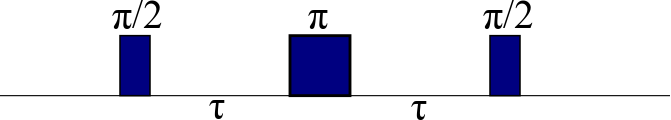
\includegraphics[scale=0.4]{Hahn1.png} 
\caption{Hahn Echo sequence: a $\pi$ pulse enclosed by two $\nicefrac{\pi}{2}$ pulses.}
\end{figure} 


\subsubsection{Decoupling sequences}\label{Ds}
Interaction with ensembles of nuclear and electron spins surrounding the NV center lead to dephasing of the NV electron spin. This mechanism can be circumvented to some extent with specific sequences which decouple the NV spin from interactions with its environment and thereby increase the coherence times. In contrast to the Hahn Echo sequence, the spin echoes are here observed after the application of multiple pulses.
\subsubsection*{Spectral decomposition of the magnetic environment}
For NV spins which are coupled to a magnetic environment, the loss of coherence can be generally described  in the form \cite{ssbd}:
\begin{equation}
C(t)=e^{-\chi(t)}
\end{equation}
where the decoherence functional is defined as
\begin{equation}\label{chi}
\chi(t)=\frac{1}{\pi}\int^{\infty}_0d\omega S(\omega)\frac{F(\omega t)}{\omega^2}
\end{equation}
Here, $S(\omega)$ is the frequency-domain spectral density of the noise, thereby describing the coupling of the system to the environment, and $F_t(\omega)$ is the filter function that represents modulations being performed on the NV spins, for example in the form of a pulse sequence.\\
It can be assumed, that the dominant source of decoherence for the NV is a bath of randomly oriented spins\cite{ssbd}. If the bath cross-correlation function has the form of a simple exponential decay, the spectral density of the noise has a Lorentzian shape:
\begin{equation}\label{SD}
S(\omega)=\frac{\Delta^2\tau_c}{\pi}\frac{1}{1+(\omega\tau_c)^2}
\end{equation}
with $\Delta$ being the average coupling strength  of the spin bath to the probed NVs and$\tau_c$ the correlation time of the N bath spins with each other which is related to their characteristic flip-flop time. With $n_{spin}$ being the N bath density, it is expected that $\Delta\propto\tau_c^{-1}\propto n_{spin}$  \cite{ssbd}.\\
The filter functions for the Hahn Echo sequence looks as follows \cite{hted}:
\begin{align}
F(z)=8\sin^4\left(\frac{z}{4}\right)
\end{align}
With the filter functions and the assumption of a Lorentzian spin bath, each data point will yield values for $\Delta$ and $\tau_c$, providing an image of the NV's magnetic environment.
A different approach can be made in the case of an ideal Dirac-delta shaped filter, where $F(\omega t)/(\omega^2t)=\delta(\omega-\omega_0)$. Then, the integral for $\chi(t)$ simply reduces to:
\begin{equation}
\chi(t)=tS(\omega_0)/\pi
\end{equation} 
thus rendering for the spectral function at frequency $\omega_0$\cite{ssbd}:
\begin{equation}
S(\omega_0)=-\pi\ln(C(t))/t
\end{equation}
\paragraph{Carr-Purcell-Meiboom-Gill sequence}\mbox{}\\
The CPMG sequence begins with a $\nicefrac{\pi}{2}$ rotation around the $y$ axis, followed by a number $n$ of ($\tau-\pi_x-\tau$) pulses with $\tau$ being the free precession time again, and ends with a $(\nicefrac{\pi}{2})_{-y}$ pulse, projecting the spin back to the bright state. The total relaxation time of the NV spin adds up to $T_{rel}=2n\tau$. The CPMG-sequence can be seen as a succession of multiple Hahn Echoes. So, because the spin is flipped more often, also higher frequencies can be suppressed, depending on the number of applied pulses. As a consequence, sequences with more pulses should achieve higher decoupling efficiencies.\\
The filter function of CPMG is of the form:
\begin{equation} F(z)=8\sin^4\left(\frac{z}{4n}\right)\sin^2\left(\frac{z}{2}\right)/\cos^2\left(\frac{z}{2n}\right)
\end{equation}
\begin{figure}[H]
\centering
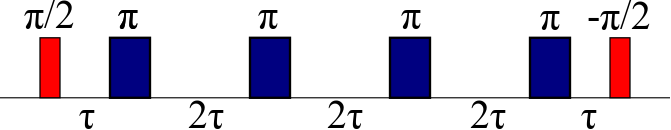
\includegraphics[scale=0.4]{CPMG41.png} 
\caption{CPMG-4 sequence: red pulses represent rotations around the y-axis, blue pulses are rotations around the x-axis}
\end{figure} 
\paragraph{XY sequence}\mbox{}\\
The XY sequences is made up of multiple $\pi_x$ and $\pi_y$ pulses. These are applied in two different variations: the asymmetric one, starting with an interval $\tau$ of free evolution and ending directly after the last pulse; and the symmetric one, which begins and ends with a $\nicefrac{\tau}{2}$ interval. The symmetric sequences have been found to achieve longer coherence times\cite{sas}\cite{sas2} and were used in the experiments for this bachelor thesis. In general, the first half of the XY-sequence consists of ($\nicefrac{\tau}{2}-\pi_x-\tau-\pi_y-\nicefrac{\tau}{2}$) pulses and in the second part, the order is inverted and the sequence continues with the same number of ($\nicefrac{\tau}{2}-\pi_y-\tau-\pi_x-\nicefrac{\tau}{2}$) pulses. As before, the sequence is enclosed by two opposite $(\nicefrac{\pi}{2})_y$ pulses. With a number $n$ of $\pi$ pulses again, the total relaxation time turns out to be $T_{rel}=n\tau$. The advantage of XY-sequences compared to CPMG is their ability to refocus the spin with pulses along different spatial directions and therefore a better performance in the presence of a general, unknown interaction \cite{dd}\cite{rdc}.
\begin{figure}[H]
\centering
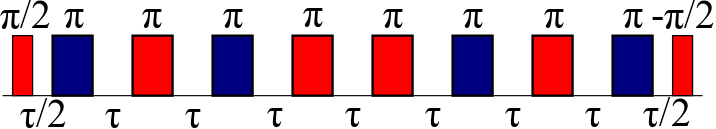
\includegraphics[scale=0.4]{XY81.png} 
\caption{XY-8 sequence, consisting of alternating $\pi_x$ and $\pi_y$ pulses. In order to form a symmetric sequence, the order of the pulses is reversed after the first half of the sequence.}
\end{figure} 
\newpage
\paragraph{UDD sequence}\label{udd}\mbox{}\\
In 2008, Uhrig stated that equidistant pulse spacings do not always produce the best results with regard to decoupling\cite{udd}. So, sequences with $n$ $\pi_x$ pulses at the time points
\begin{equation}\label{udde}
\delta_j=\tau\sin^2\left(\frac{\pi j}{2n+2}\right)
\end{equation}
have proven to achieve the optimum suppression of decoherence caused by imperfect pulses. Furthermore, they perform also well with regard to the decoupling from a spin bath \cite{udd}. Between the two required $(\nicefrac{\pi}{2})_y$ pulses, the sequence is symmetric with increasing time intervals to the middle and decreasing spacings to the end. The total free spin relaxation time of UDD is just $\tau$.\\
The UDD filter function is:
\begin{equation}
F(z)=\frac{1}{2}\left|\sum^n_{k=-n-1}(-1)^k\exp\left(\frac{iz}{2}\cos\left(\frac{\pi k}{n+1}\right)\right)\right|^2
\end{equation}
\begin{figure}[H]
\centering
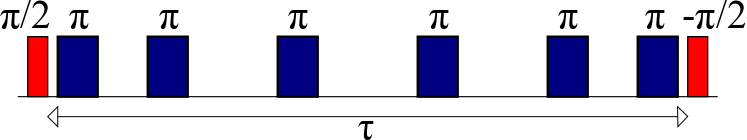
\includegraphics[scale=0.4]{UDD1.png} 
\caption{UDD-6 sequence: the intervals between the pulses are increasing at the beginning and decreasing after half of the pulses, resulting in a symmetric sequence.}
\end{figure} 

\section{Experimental realization}
In the following section the experimental details and procedures will be explained. After describing the setup, the principle of confocal microscopy will be discussed further. At the end, the calibration of the components will be briefly presented. 
\subsection{Experimental setup}
\subsubsection{Optical setup}
The first component of the setup is a 532 nm Laser that drives the NV optical transitions and is used to initialize the spin to $m_s=0$ and perform the spin readout via fluorescence measurement. The Laser can be pulsed with an AOM with rise/fall times of approximately 50 ns. After that, the light goes through a 532 nm shortpass, creating a beam of the preferred wavelength. The next element is a dichroic mirror (DM) which reflects light below 600 nm and transmits light above that wavelength. After the DM, the beam goes into the microscope and gets focused onto the sample by means of an oil immersion objective lens with a numerical aperture of NA = 1.35. Two different samples have been used in the experiments. The first sample was prepared by spin coating a solution of 25 nm large type Ib nanodiamonds on a glass substrate (Microdiamant AG - QP25). The second sample was a type IIa Bulk diamond with a size of 2x2x0.05 mm. It was produced via CVD and implanted with nitrogen, resulting in an NV density of more than 10 NVs/focal point. The samples are mounted onto a piezo-controlled xyz stage that allows the adjustment of the sample-to-objective distance. A microwave antenna is placed above the sample, allowing us to conduct ESR measurements and run decoupling sequences. The photons emitted by the NVs are collected with the lens before leaving the microscope. At the DM, the red PL gets transmitted. A long pass filter removes residual Laser light, before the beam goes into the confocal part that is made up of two collecting lenses and a pinhole in between.
At the end, the light reaches the APD and gets detected. Ideally, the last part of the setup would be a Hanbury-Brown and Twiss (HBT) setup to make autocorrelation measurements. This consists of a beam splitter, which has a 50:50 probability of either reflecting or transmitting the photons, and two APDs for counting the reflected and transmitted photons, respectively. This arrangement is also shown in the conceptual setup scheme.\\
Since the APD signals shouldn't be acquired all the time the APDs are gated. This means, that the detected intensity is only read out, when the gates are open. There are two gates: the reference gate (ref), which is open before the spin manipulation took place and the signal gate (sig) which is open at the end of the sequence. Their quotient sig/ref yields the normalized intensity. \\
The laser and the APD gates are controlled by a bit pattern generator with a minimum pulse length of 6.6 ns.
\subsubsection{Microwave setup}
For the purpose of doing various ESR measurements on the NVs, it was essential to use two different microwaves with a relative phase shift of 90$^\circ$. This could be accomplished in an additional part of the setup. At first, the signal of the RF generator gets into a 0$^\circ$-90$^\circ$ RF power splitter. Then, each separate signal goes through a switch that is controlled via TTL pulses from the bit pattern generator. Finally, the signals from both switches are recombined in a simple RF power combiner and transmitted to the microwave antenna. A setup scheme is depicted in figure \ref{setup}.
\begin{figure}[H]
\centering
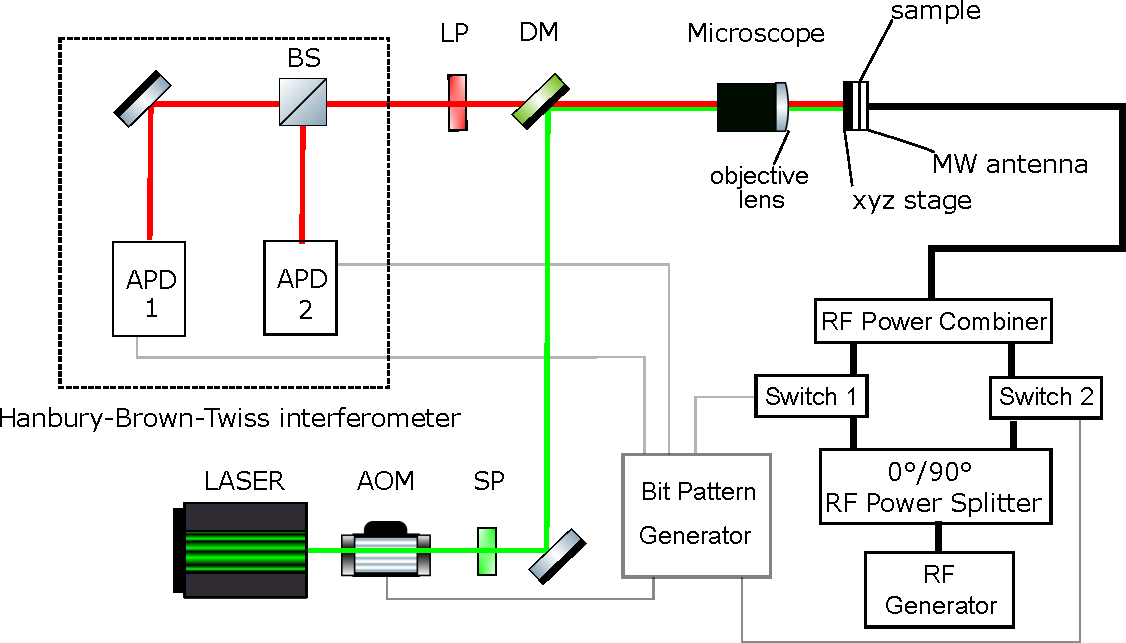
\includegraphics[scale=0.7]{setup4.pdf} 
\caption{Schematic image of the conceptual experimental setup: instead of the HBT part, the actual setup just contains an APD.}
\label{setup}
\end{figure}

\subsection{Confocal microscopy}
A conventional microscope collects light from any photon source in the sample, regardless of whether it originates from the focal plane or not and thus leads to a reduction in contrast and sharpness of the image. The advantage of a confocal microscope is, that it doesn't only achieve a high 2-D resolution but is also able to suppress light which doesn't come from the focal plane. This can be achieved with a pinhole in the confocal plane. In our setup, it was implemented by putting two lenses in the beam path and placing the pinhole in the common focal plane of the two lenses. As only the photons that go through the pinhole are detected, light from below or above the focal plane is extinguished. So, this arrangement accomplishes depth discrimination as shown in figure \ref{cmz}.
\begin{figure}[H]
\centering
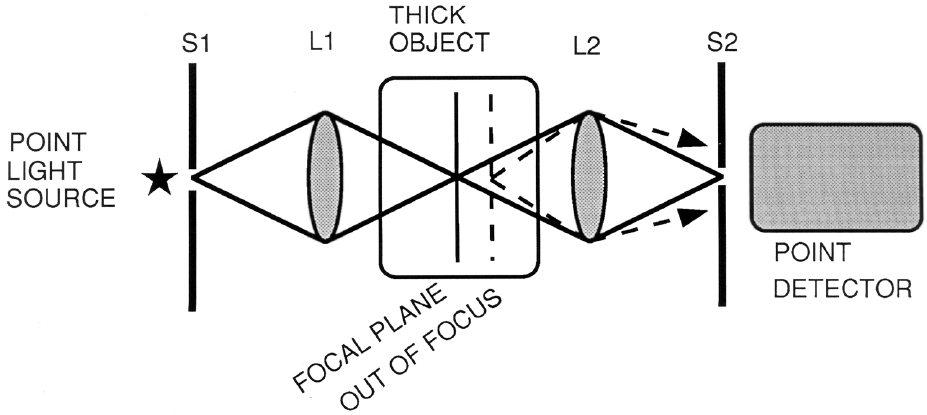
\includegraphics[scale=0.4]{cmzfocus.png} 
\caption{Schematic image of the confocal part of the setup, illustrating depth discrimination with the dashed beams. This image was taken from \cite{cmmem}.}
\label{cmz}
\end{figure}
Obviously, the degree of depth discrimination depends on the size of the pinhole and can consequently be modified by changing the diameter of this aperture. However, in our experiments we used a pinhole which was around 1 Airy disk diameter; this size will be estimated in the next section. Furthermore, the confocal part also filters out stray light, hence enhancing the contrast\cite{czj}.
\\
\subsubsection{Point Spread Function}
Due to diffraction effects, light that comes from a point-like object in the focal plane doesn't converge to a single point in the image plane. It rather spreads slightly in all directions, even in a diffraction-limited system, where all optical components have ideal properties and are perfectly adjusted. In confocal fluorescence microscopy, this phenomenon occurs actually twice: the laser light cannot be ideally focused onto the sample, and the emitted light cannot be perfectly focused on the pinhole. The image of a single point can be described by the point spread function (PSF), which accordingly contains information about the highest possible resolution. Since the confocal microscope enables imaging in three dimensions, it is necessary to consider the 3-D PSF, which appears to be a rotational ellipsoid:
\begin{figure}[H]
\centering
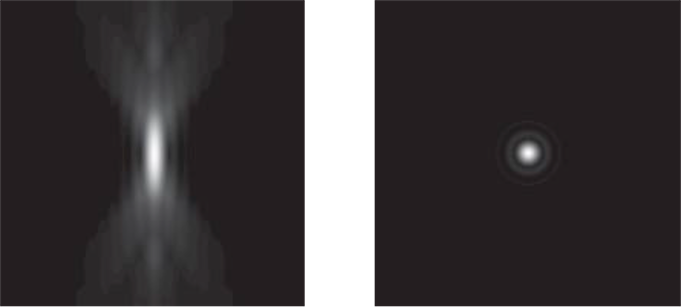
\includegraphics[scale=0.5]{PSF.png} 
\caption{Slices through the 3-D PSF. The left image shows the intensity distribution in axial direction and the right image shows a lateral plane. These images were taken from\cite{czj}.}
\label{psf}
\end{figure}
According to the Rayleigh-criterion, "two components of equal intensity should be considered to be just resolved when the principal intensity maximum of one coincides with the first intensity minimum of the other"\cite{poo}. Naturally, resolution is also affected by the signal-to-noise ratio of the system\cite{cfm}, so this criterion cannot be applied in every case. The distance to the first minimum corresponds to the radius of the Airy disk, giving for the minimum distance between two resolvable objects:
\begin{equation}
d_{min}=\frac{1}{2}AU=\frac{0.61\sqrt{\lambda_{ex}\lambda_{em}}}{NA}\approx\unit[236]{nm}
\end{equation}
with $\lambda_{ex}$ being the excitation and $\lambda_{em}$ the emission wavelength, respectively. AU (Airy Unit) denotes the diameter of the Airy disk, NA is the numerical aperture of the lens. 
Taking the magnification $M=60$ of the objective into account, the pinhole diameter can be calculated:
\begin{equation}
d_{ph}=\frac{1.22\sqrt{\lambda_{ex}\lambda_{em}}}{NA}M\approx\unit[30]{\mu m}
\end{equation}
This pinhole size was used in the experiments.
\subsection{Calibration}
Due to differences in the response times of each device and cable delay effects, a signal generated by the bit pattern generator at a specific moment would lead to an outcome at a different time for each component. Consequently, the sequence which is output by the BPG is executed in a completely different way, making it essential to adjust the timing of each element. As just the relative delays of the components to each other needed to be adapted, the delay of the laser was set to zero and the other delays were determined with respect to the laser.
\subsubsection{Calibration of the APD gates}
To calibrate the gates, the microscope was initially focused on an NV. Then, the laser was switched on for a short period of time, thereby exciting the NV and producing fluorescence. Simultaneously, the signal and reference gates detected the intensity over the same timespan but with different delays regarding the laser. By plotting the signal over reference ratio, it is clear that the unity level is reached  when the two respective detection windows superimpose, providing the corresponding delay times.
\begin{figure}[H]
\centering
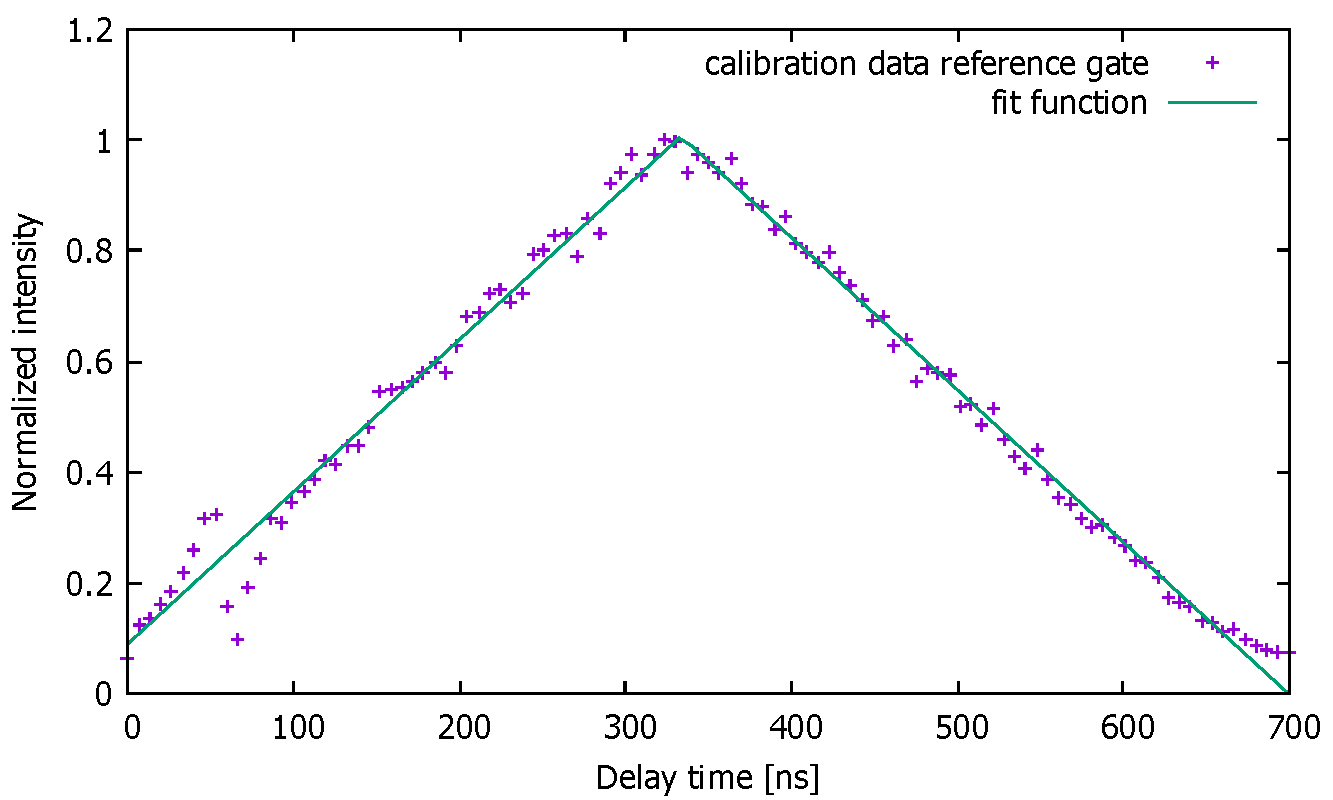
\includegraphics[scale=0.5]{gatestiming.pdf} 
\caption{Measurement of the normalized intensity(divided by the maximum value) in dependence of the gate position regarding the laser; the peak of the graph yields the time delay.}
\label{gt}
\end{figure}
\subsubsection{Calibration of the microwaves}
For the calibration of the microwaves, the laser was turned on for the duration $T$ of the sequence, driving the NV to $m_s=1$. Additionally, a MW pulse of length $\tau$ was applied at time $t$, the reference was measured from $\nicefrac{T}{2}-\tau$ until $\nicefrac{T}{2}$ and the signal directly after that, from $\nicefrac{T}{2}$ to $\nicefrac{T}{2}+\tau$. Then, the signals were measured for different $t$ from 0 to $T-\tau$, shifting the pulse through the sequence. For small $t$, the normalized intensity would be 1, as the NV is driven back to the excited state by the laser. When $t$ increases further, the counts measured in the reference gate decrease, resulting in a normalized intensity above 1. 
\begin{figure}[h!]
\centering
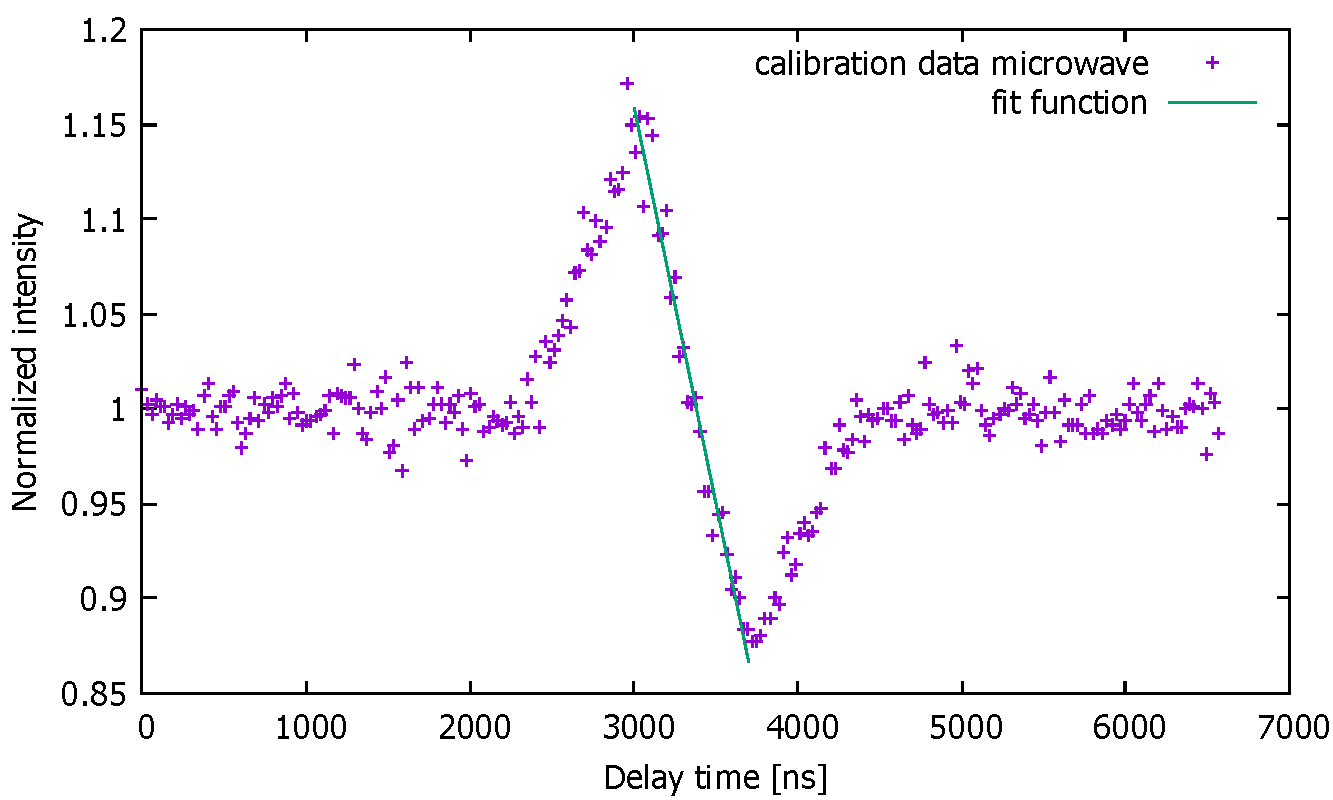
\includegraphics[scale=0.5]{mwt.pdf} 
\caption{Measurement of the normalized intensity as a function of the mw pulse position}
\label{mwt}
\end{figure}
\newpage
When the microwave pulse is exactly between the two gates, the normalized intensity reaches 1 again and afterwards, the image is the same as before, just vice versa. So, the microwave is timed correctly, when the normalized intensity goes to 1 exactly at $\nicefrac{T}{2}$.


\section{Measurements}
In order to lift the degeneracy of the $m_s=\pm1$ sublevels of the NV, a static magnetic field was applied on the sample. After optically identifying the appropriate NV or the relevant measurement spot in case of the bulk diamond, an RF scan was performed to characterize the defect's resonance. With a Hanbury-Brown and Twiss setup, an autocorrelation function (see chapter \ref{g2}) was sufficient to prove that a single NV was in the confocal volume. However, when the HBT was not available, only a good estimation based on the fluorescence intensity level and the RF scan and line-widths could be made.
 For the ensuing measurements it was necessary to determine the resonant frequencies as accurately as possible. Therefore, the RF scan data were fit with a double-Lorentzian function of the form:
\begin{equation}
I(\omega)=C_0+\frac{C_{11}}{C_{12}+(\omega-\omega_1)^2}+ \frac{C_{21}}{C_{22}+(\omega-\omega_2)^2}
\end{equation}  
The RF scan was followed by the Rabi sequence. So as to make sure that both microwaves had the same power, the Rabi sequence was performed with each MW phase separately. As mentioned in section \ref{DM}, the data were fit with a product function of sine and cosine. After that, a Hahn Echo was acquired to determine the dephasing time without decoupling pulses. Then, the decoupling sequences could be executed. 
\subsection{Examination of single NVs in nanodiamond}
The first measurements were conducted on the nanodiamonds. With an NV density of about 1 per 10($\mu$m)$^2$, we were able to focus the microscope on single NVs and study their properties.
\subsubsection{Resonance scan and Rabi oscillations}
The process of finding a suitable NV for the measurement included focusing on multiple NVs and making RF scans. When the contrast was sufficiently high - meaning an intensity difference of at least 15\% during the scan - and the resonance dips were more than 50 MHz apart and therefore easily separable, the NV could be considered suitable. A suitable NV center would hence show the resonance spectrum displayed in figure \ref{rf2}.
\begin{figure}[H]
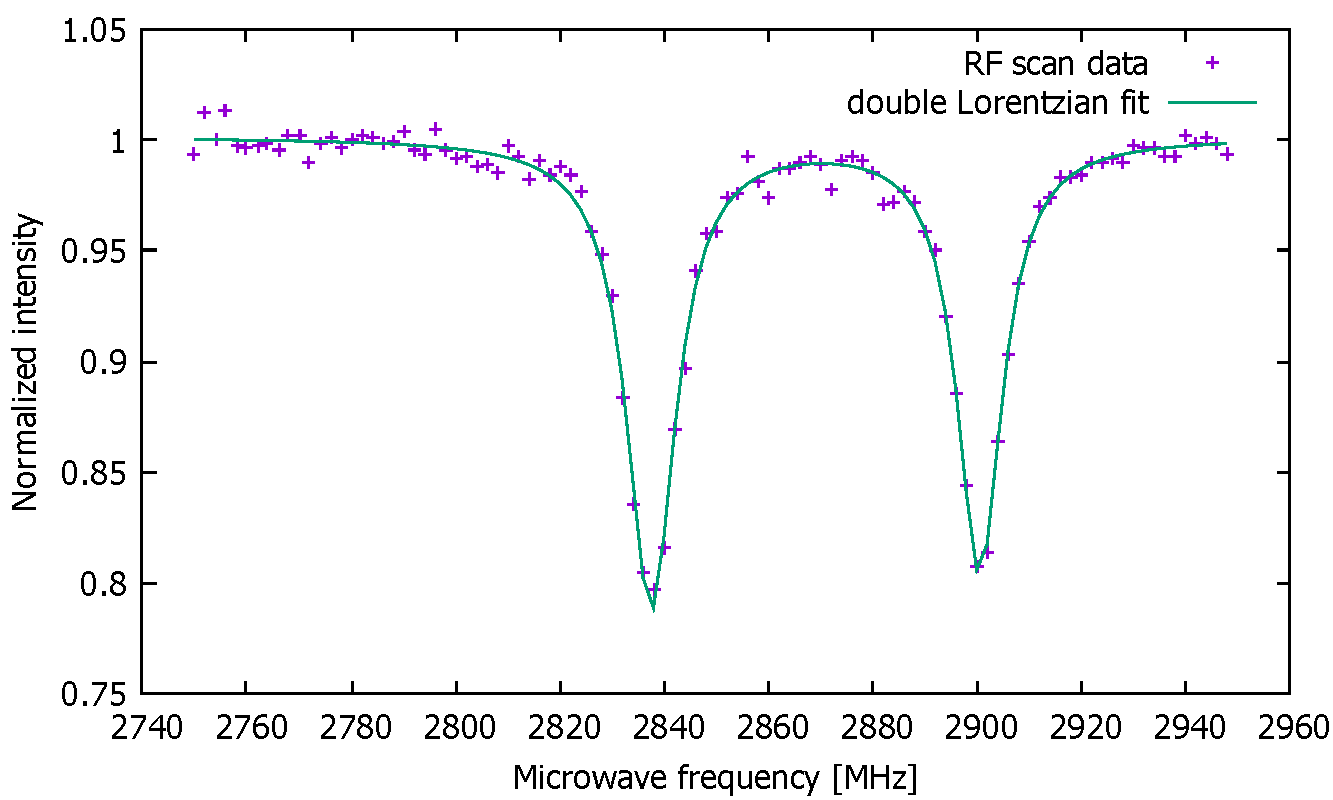
\includegraphics[scale=0.6]{rf2fit.pdf} 
\caption{Rf scan, showing a separation of 60 MHz of the resonant transitions. The data were fit with a double-Lorentzian}
\label{rf2}
\end{figure}
In absence of off diagonal elements of the matrices in equation (\ref{hz}), the $m_s=+1$ and $m_s=-1$ levels exhibit equal properties. We therefore choose to work in the $m_s=0$, $m_s=-1$ subspace, where the energy difference between the two basis states is $\nu=\unit[2837.5]{MHz}$.
\\
By driving Rabi oscillations on the $m_s=0$ to the $m_s=-1$ transition with the selected microwave power, we deduce a $\nicefrac{\pi}{2}$ pulse length of $t_{\pi/2}=\unit[45.6]{ns}$. \\
\begin{figure}[H]
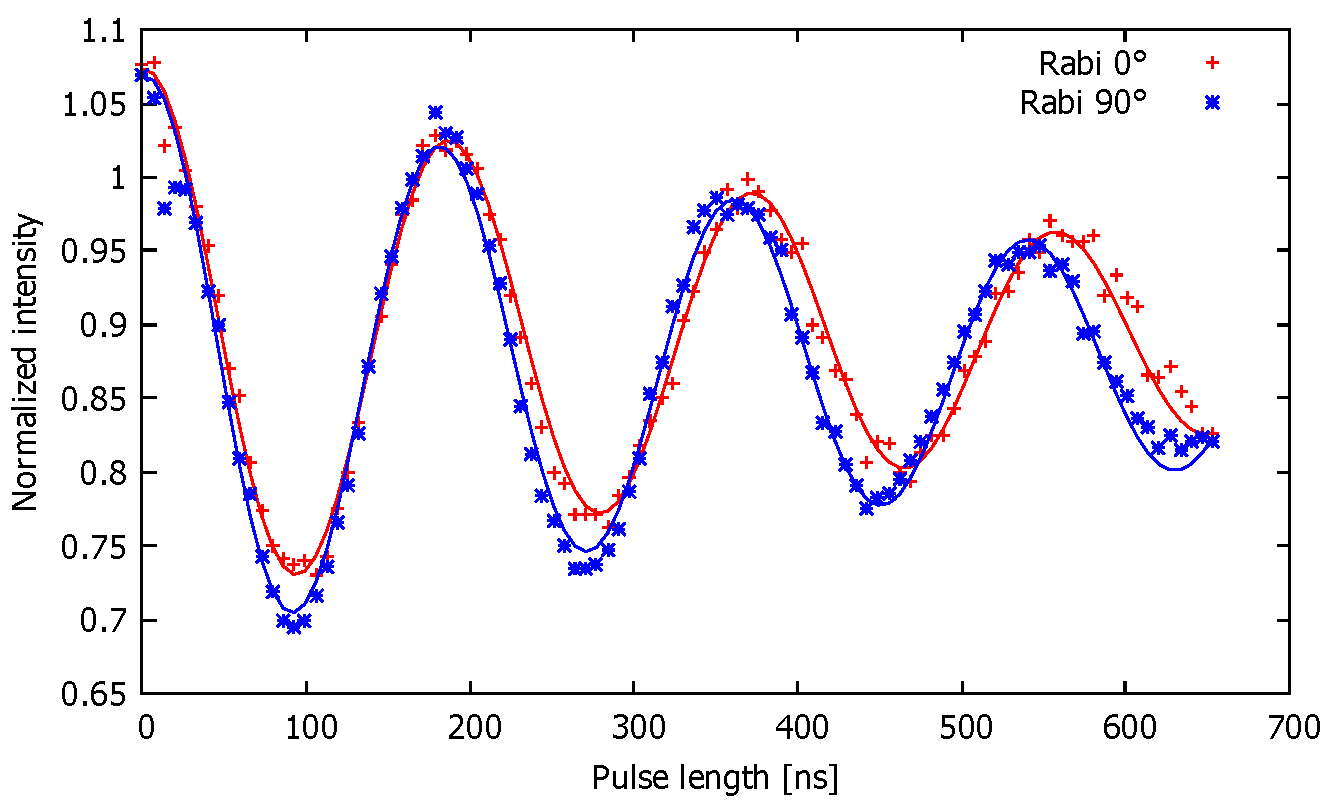
\includegraphics[scale=0.6]{rabinano.pdf} 
\caption{Rabi oscillations for normal and phase-shifted MW. The data were fit with a function of the form $I(t)=C_1\cdot\exp(\gamma(t-t_0))\cdot\cos\left(\frac{\pi(t-t_0)}{2t_{\pi/2}}\right)+C_2$.}
\label{rabn1}
\end{figure}
With this knowledge, spin manipulation measurements could now be executed. 
\subsubsection{Decoupling sequences}
At first, a Hahn Echo sequence was executed to measure the NV's $T_2$ time.
\begin{figure}[H]
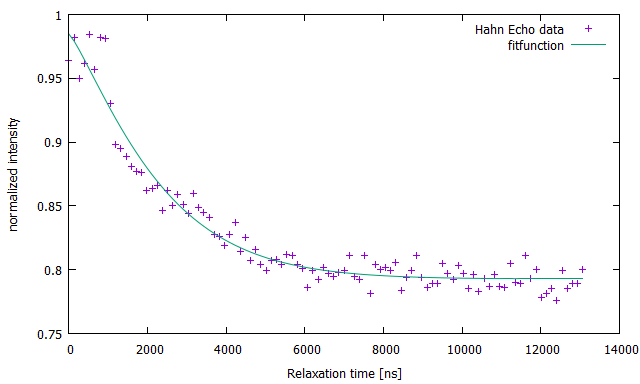
\includegraphics[scale=0.6]{Hahnn110.pdf} 
\caption{Hahn Echo measurement, exhibiting a simple exponential decay.}
\label{H1}
\end{figure}
The exponential decay of the spin echoes was fit with an exponential function of the form
\begin{equation}\label{exp}
I(t)=c_1e^{-\left(\frac{t}{t_0}\right)^\alpha}+c_2
\end{equation}
with $t_0$ being the coherence time. In theory, the exponent $\alpha$ is related to the spectral density function. For a Lorentzian shape spin bath, theoretical models predict $2\leq\alpha\leq3$\cite{ess}. However, it was shown that fits with different values of $\alpha$ give equally good results, independent of the coherence time\cite{sdd}. For this reason, $\alpha$ gives little information about the spin bath and will be considered as a fitting parameter. \\
The Hahn Echo (figure \ref{H1}) gives for the relaxation time $T_2=t_0=\unit[2.41\pm 0.12]{\mu s}$. 
\\
The setup only allowed to apply $0^\circ$ or $90^\circ$ microwave pulses. Consequently, instead of a final $\nicefrac{\pi}{2}_{-y}$ pulse, we could only generate a $\nicefrac{3\pi}{2}_y$ pulse to project the spin onto the bright state. Another possibility, which was used in the nanodiamond measurements, was to end the sequence with another $\nicefrac{\pi}{2}$ pulse that would project the spin onto the dark state of the NV. The advantage of this approach is that the last MW pulse is much shorter and the pulse errors have a smaller impact on the measurement, resulting in a higher contrast. Considering that the populations of bright and dark state are inverted with respect to each other, the behaviour of the data curves will also be inverted to what one would get using the correct realization of the sequences. However, this is a matter of convenience and doesn't change the physical meaning of the measurements.
\paragraph{CPMG}\mbox{}\\
The CPMG-sequence has been examined for 8, 16, 32 and 64 $\pi$ pulses. It would have been possible to do measurements with less pulses, but as the shortest symmetric XY-sequence is XY-8, the data wouldn't have been comparable to other sequences.\\
\begin{figure}[H]
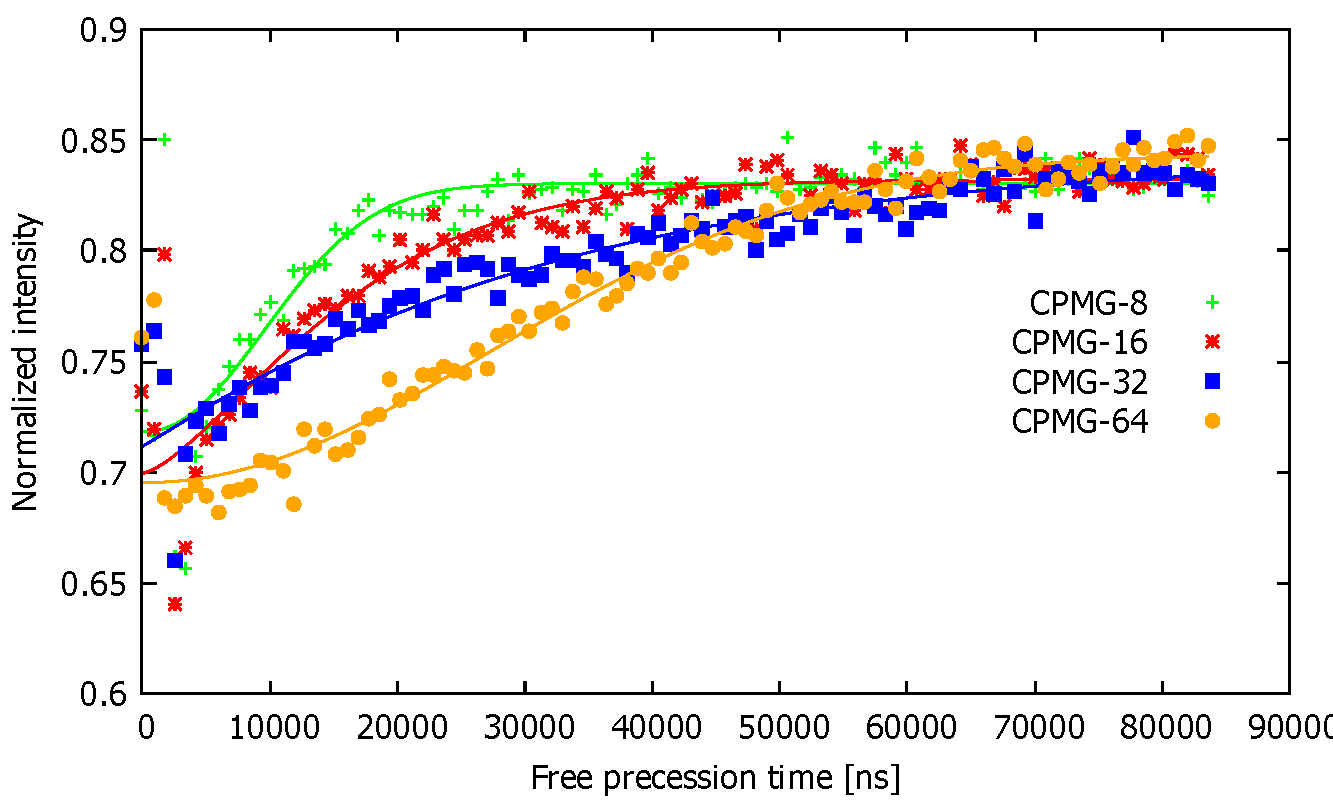
\includegraphics[scale=0.6]{4cpmgo1pt.pdf} 
\caption{Comparison of CPMG-sequences with different numbers of pulses. The solid lines are fits to the data points made using the model in equation (\ref{exp}). It can be seen that the coherence time increases with the number of pulses.}
\label{C4}
\end{figure}
From a qualitative point of view, the curves in figure \ref{C4} show the expected behaviour: the more pulses are applied, the slower is the intensity decay. This observation is supported by the fits which were made with the function presented in equation (\ref{exp})(the fit data are shown in table \ref{ct}). The exponent $\alpha$ shows no consistent behaviour throughout the sequences. \\
Apart from that does the coherence time show the predicted behaviour: it rises gradually with the number of $\pi$-pulses and gets as far as almost 16 times the relaxation time.\\
\begin{table}[H]
\centering
\caption{Exponential behaviour and coherence times for different numbers of pulses}
\label{ct}
\begin{tabular}{l|ll|l}
sequence & exponent $\alpha$             & $t_0$ {[}ns{]}  & $t_0/T_2$                     \\\hline
CPMG-8   & 2.13  $\pm$ 0.53 & 12900           $\pm$ 1100 & 5.35\\
CPMG-16  & 1.42  $\pm$ 0.22 & 17500            $\pm$ 1400 &7.26\\
CPMG-32  & 1.06  $\pm$ 0.19 & 31700         $\pm$ 3700 & 13.14\\
CPMG-64  & 2.03  $\pm$ 0.17  & 38100        $\pm$ 1200 & 15.80
\end{tabular}
\end{table}
By having NV centers embedded in nanosized crystals it is legitimate to assume that the spin bath contribution may have a component related to the bare crystal impurities and a component related to surface effects. Hence, it is to expect that NVs in different nanodiamonds would show different behaviours under dynamical decoupling. This effect has  been observed by repeating the CPMG-8 and  Hahn Echo sequences on few nitrogen vacancies in different nanodiamonds. The result of these measurements can be seen in figure \ref{C8}.
\\
From Hahn Echoes of various NVs, we got transverse relaxation times $T_2$ in the range between 250 ns and 2.5 ms. The CPMG sequence was conducted for NVs with $\unit[0.9]{ms}\leq T_2\leq\unit[2.4]{ms}$. 
\begin{figure}[H]
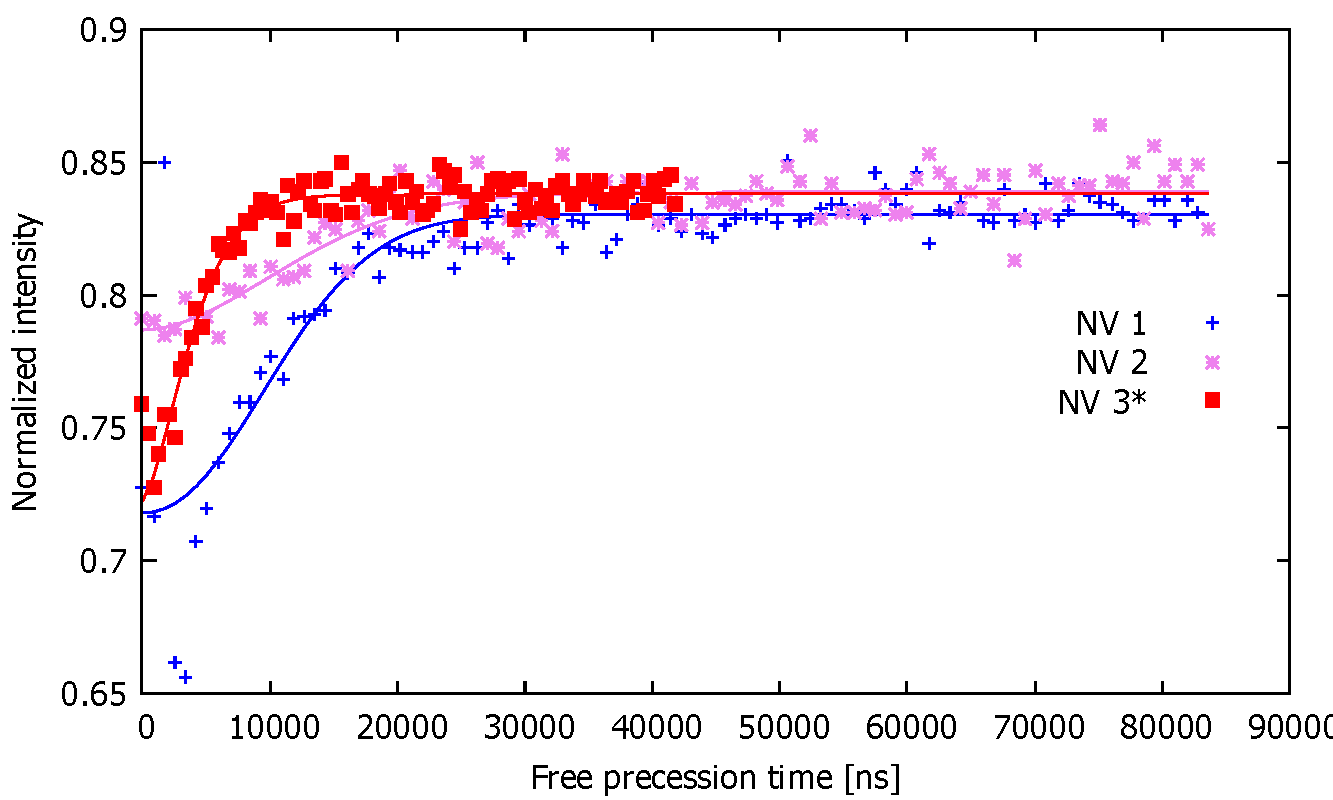
\includegraphics[scale=0.6]{cv.pdf} 
\caption{Comparison of CPMG-8 sequences for different NVs with $T_2$ times ranging from 0.9 ms (NV 3) to 2.4 ms (NV 1). For a better comparability, the data of NV 3 were modified by an offset of 0.1. The data have been fit with an exponential function as described in equation (\ref{exp}).}
\label{C8}
\end{figure}
It can be seen that the same decoupling sequence achieves different coherence times depending on the specific properties of the NV. The contrast seems to have no effect on the performance of the sequence.\\
\begin{table}[H]
\centering
\caption{Exponential behaviour and coherence times of CPMG-8 for different NVs}
\label{cv}
\begin{tabular}{l|ll|l}
&exponent $\alpha$ & $t_0$ {[}ns{]}                     & $t_0$/$T_2$             \\\hline
NV 1            & 2.13          $\pm$ 0.53 & 12900            $\pm$ 1100         & 5.35 \\
NV 2            & 1.76         $\pm$ 0.17  & 5000           $\pm$ 200       & 3.45 \\
NV 3            & 1.89         $\pm$ 0.49 & 14700         $\pm$ 1400         & 16.63
\end{tabular}
\end{table}
The fit data(table \ref{cv}) exhibit a consistency with regard to the exponential behaviour: all values of $\alpha$ lie in the range $2\pm0.3$.  
\\
The development of the coherence times under CPMG-8 manipulation is less consistent, however. All coherence times are increasing, but the extent of the enhancement varies greatly. The quotient of coherence and the NV's $T_2$ time, representing something like a "degree of decoupling", ranges from 3.5 to over 16 and thereby differs by a factor 5. This implies different spectral densities of the coupling of the NV electron spin to the environment and underlines the previously stated dependency of the decoupling efficiency on the individual properties of the NV.
\paragraph{XY}\mbox{}\\
Analogously to CPMG, The XY-sequence has been performed with 8, 16, 32 and 64 pulses. Due to likey AOM-related effects, the data could only be fit up to total free precession times of 40$\mu s$.
\begin{figure}[H] 
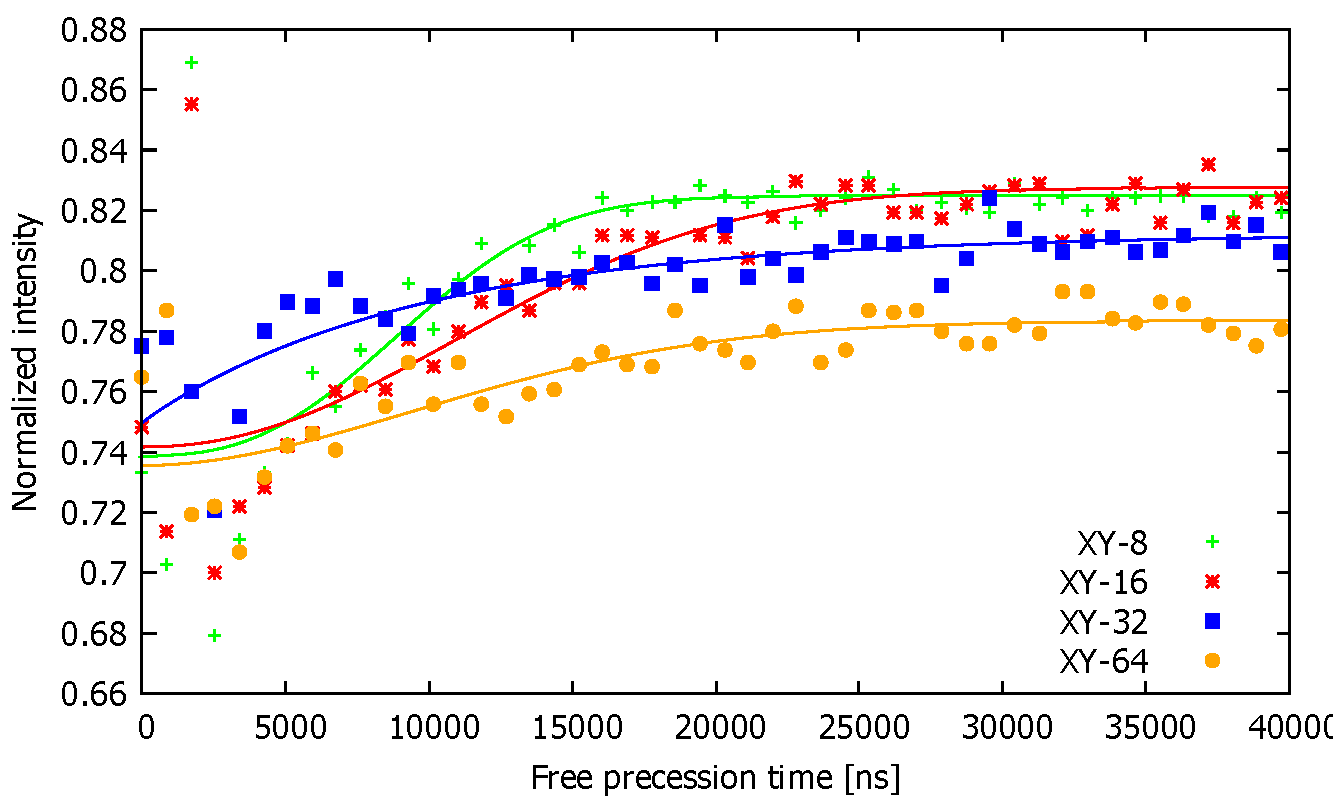
\includegraphics[scale=0.6]{nanox.pdf} 
\caption{Comparison of the XY-sequence for different numbers of $\pi$ pulses. The sequence with 16 pulses has improved the coherence time with respect to XY-8. The sequences with more pulses deviate from this trend and show an abnormal behaviour. The data have been fit with an exponential function as described in equation (\ref{exp}).}
\label{X4}
\end{figure}
The plot shows that XY-8 and XY-16 behave similarly as the CPMG sequences with the same numbers of pulses. However, the tendency doesn't continue for higher numbers of pulses: XY-32 and XY-64 exhibit great discrepancies regarding the sequences with fewer pulses. This is also underlined by the fit parameters. The first two sequences could achieve an improvement up to 6 times the $T_2$ time, but as the sequences with more pulses don't achieve longer coherence times, this is the best that could be accomplished with XY sequences for this specific NV. Furthermore, the decreasing exponent $\alpha$ has been observed here as well as for CMPG.\\               
\begin{table}[H]
\centering
\caption{Exponential behaviour and coherence times for XY}
\label{xyt}
\begin{tabular}{l|ll|l}
sequence&	exponent $\alpha$&	$t_0$ {[}ns{]}	&$t_0/T_2$\\\hline
XY-8	&2.73         $\pm$ 1.40 &	10400          $\pm$ 1400&	4.33\\
XY-16&	2.53         $\pm$ 1.04	&13700          $\pm$1600	&5.68\\
XY-32&	1.17         $\pm$ 0.51&	9900        $\pm$ 2400& 	4.09\\
XY-64&	1.83        $\pm$ 0.77	&14000         $\pm$ 2200&	5.79\\
\end{tabular}
\end{table}

The comparison of XY-8 for different NVs leads to similar observations as with the CPMG sequence.\\
\begin{figure}[H] 
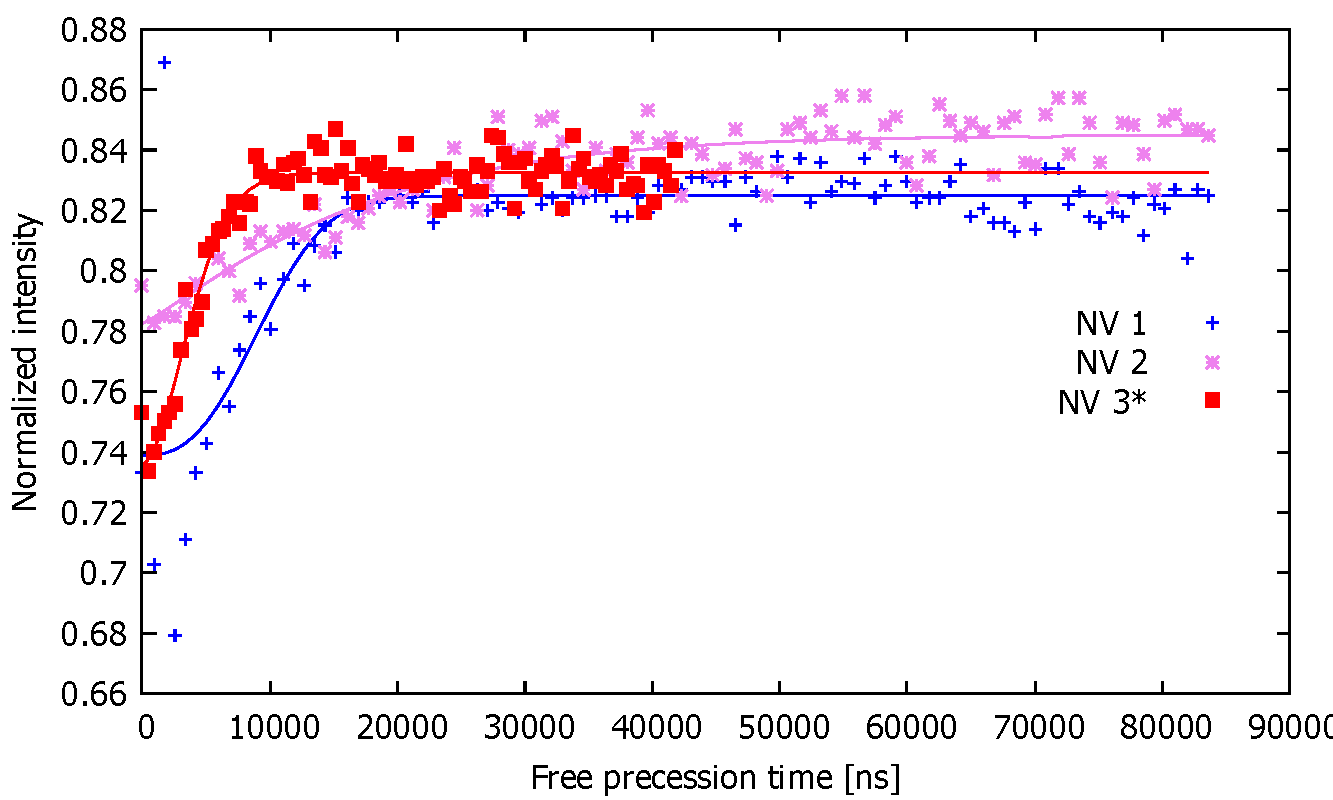
\includegraphics[scale=0.6]{xv.pdf} 
\caption{Comparison of XY-8 sequences for different NVs with $T_2$ times ranging from 0.9 ms (NV 3) to 2.4 ms (NV 1). Again, the data of NV 3 were modified by an offset of 0.1. The data have been fit with an exponential function as described in equation (\ref{exp}).}
\label{X8}
\end{figure}
In fact, XY-8 performs best for NV 3, as it was the case for CPMG-8. Here, an improvement of factor 19 could be accomplished. For the other NVs, XY-8 gave slightly worse results for the $T_2$ time.\\
\begin{table}[H]
\centering
\caption{Fit parameters of XY-8 for different NVs}
\label{X8t}
\begin{tabular}{l|ll|l}
& exponent $\alpha$ & $t_0$ {[}ns{]}                                              & $t_0$/$T_2$              \\\hline
NV 1            & 2.62         $\pm$ 0.90 & 10700         $\pm$ 1000         & 4.42 \\
NV 2            & 1.74         $\pm$ 0.20 & 4600         $\pm$ 200        & 3.18 \\
NV 3            & 1.15          $\pm$ 0.24 & 17000        $\pm$ 2000         & 19.42
\end{tabular}
\end{table}
In contrast to the CPMG fit data, the exponent $\alpha$ varies greatly between the different NVs.
All in all, this leads to the conclusion that the dynamics underlying the decay of the spin state are more complex than predicted by theory and $\alpha$ doesn't provide a complete picture about the NV center's environment.\\
Summarizing the measurements for the different NVs, one can say that although the extent of coherence time enhancement depends on the decoupling sequence, the actual achievable coherence time depends in particular on the chosen NV.
\paragraph{UDD}\mbox{}\\
The concrete way of implementing UDD showed more challenges than the other decoupling sequences. As CPMG and XY are characterized by equidistant pulse spacings, it makes no difference whether to consider the intervals between the edges of the pulses or between the centers of the pulses. This is not the case for UDD, because the intervals between consecutive $\pi$ pulses are time dependent. For that reason, UDD was implemented in two ways. The first method had edge-to-edge spacings as described in paragraph \ref{udd} equation (\ref{udde}), the second one arranged the centers of pulses according to this relation. It should be remarked that both approaches are reasonable, because the derivation of the UDD pulse spacings is based on the assumption of perfect $\delta$ pulses \cite{udd}. Obviously, for $t(\pi)\rightarrow 0$, both options are equal.\\
The graph displays an enhancement of the relaxation time through UDD, actually almost similar to the effect of XY-8 and CPMG-8. The downside, however, are the great fluctuations of the data points even for long relaxation times. This effect intensifies further for sequences with more pulses, which is why only UDD with 8 pulses could be applied successfully. A possible reason for the great variation is the limited resolution of the bit pattern generator: the implementation of UDD gets incorrect since the pulse positions have to be approximated to the 6.6 ns time steps allowed by the electronics.
\\
\begin{figure}[H] 
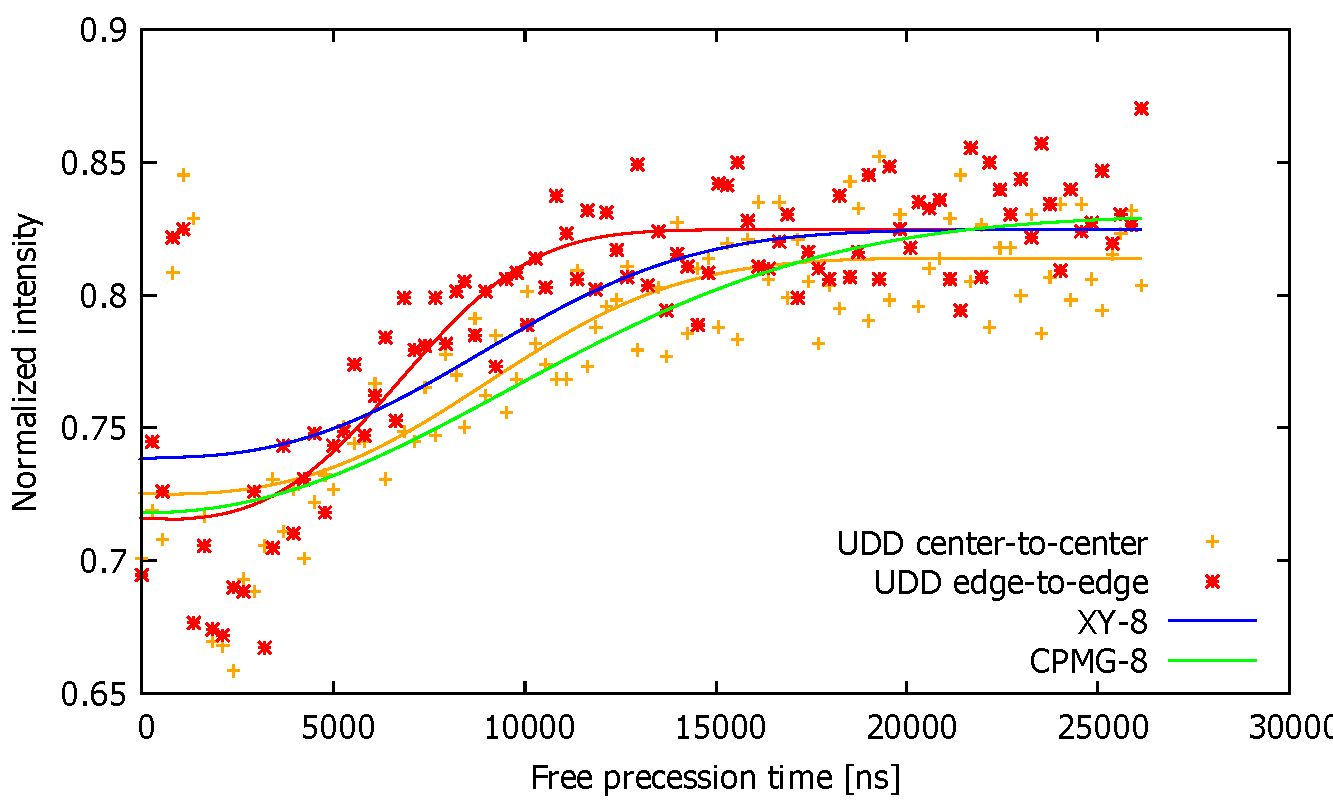
\includegraphics[scale=0.6]{udd8.pdf} 
\caption{UDD-8 sequences in two different configurations. For comparison, the fit curves of XY-8 and CPMG-8 are included in the graph. The center-to-center pulse spacings achieve a higher coherence time than the second alternative. The improvement of $T_2$ is comparable to the other decoupling sequences, but the data points are scattered more widely. The data have been fit with an exponential function as described in equation (\ref{exp}).}
\label{U8}
\end{figure}
It can be seen that UDD-8 with center-to-center pulse spacings gives a higher coherence time than the second sequence. This is confirmed by the fit parameters in table \ref{U8t}: $t_0$ is almost 3 $\mu$s higher for the first implementation and even matches the value for XY-8.\\
\begin{table}[H]
\centering
\caption{Comparison of both UDD-8 sequences with CPMG-8 and XY-8}
\label{U8t}
\begin{tabular}{l|ll|l}
& exponent $\alpha$ & $t_0$   {[}ns{]}                                                   & $t_0$/$T_2$              \\\hline
UDD-8 center-to-center       & 2.81           $\pm$ 0.90 & 10600          $\pm$ 900        & 4.39 \\
UDD-8 edge-to-edge       & 2.95          $\pm$ 0.80  & 7700          $\pm$ 500        & 3.22\\
CPMG-8          & 2.13          $\pm$ 0.53 & 12900            $\pm$ 1100         & 5.35 \\
XY-8            & 2.62          $\pm$ 0.90 & 10700          $\pm$ 1000          & 4.42       
\end{tabular}
\end{table}

\paragraph{Comparison of XY and CPMG}
In the literature relating to NV centers in bulk diamond, CPMG was found to perform better than XY sequences of equal pulse number\cite{dd}. It is now interesting to find out if this is also the case for nanodiamonds.
\begin{figure}[H] 
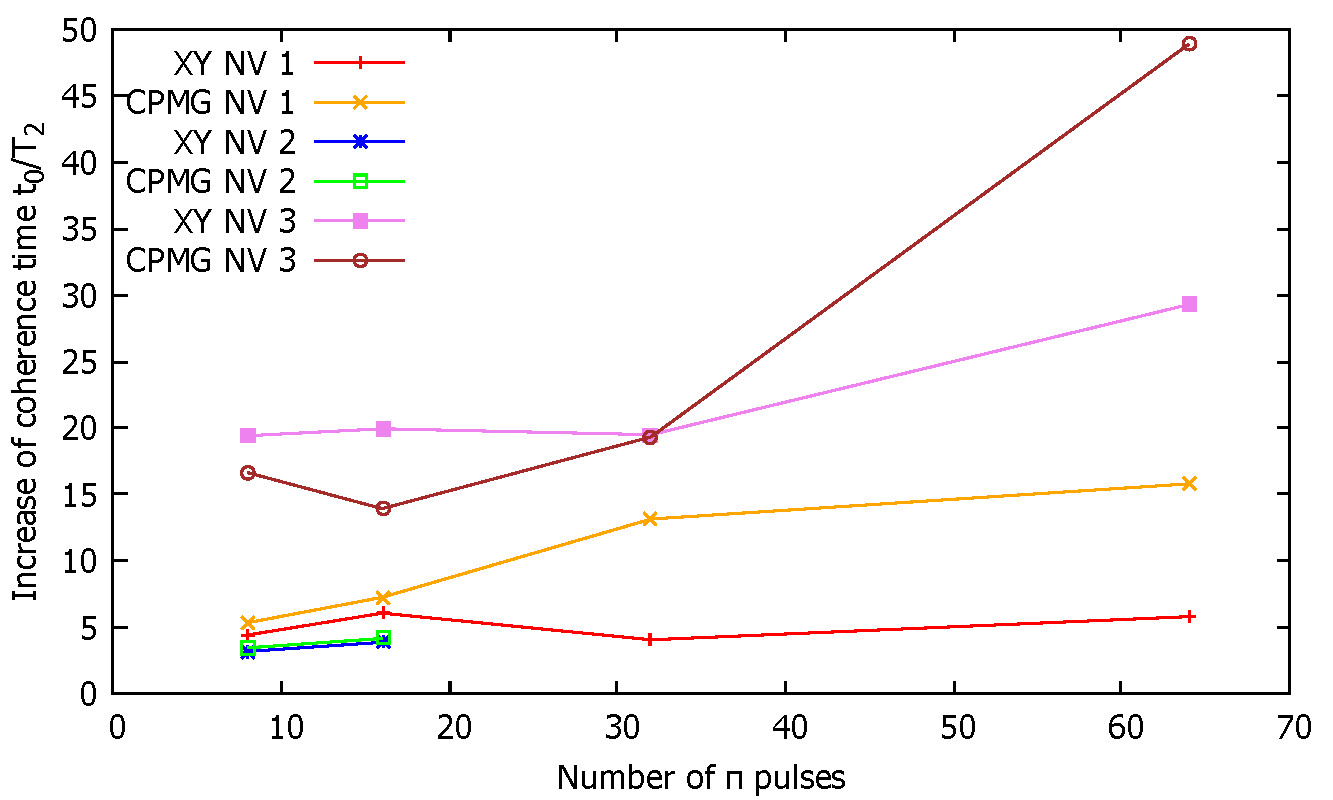
\includegraphics[scale=0.6]{xcvergleich.pdf} 
\caption{Extension of the relaxation time, quantified by the quotient $t_0/T_2$, as a function of the number of $\pi$ pulses for XY and CPMG sequences in different NVs. For 8 and 16 pulses, both sequences perform equally well; when more than 16 pulses are applied, CPMG gives better results, achieving an enhancement of up to 50 times $T_2$.}
\label{xc}
\end{figure}
It turns out that both sequence types reach similar coherence times for 8 and 16 pulses, XY performing slightly better than CPMG for the third NV. Regarding the sequences with more pulses, CPMG could achieve longer coherence times than XY, even for NV 3, where the short sequences performed worse than XY.
\subsubsection{Spectral decomposition}
As discussed in section \ref{Ds}, the decay of coherence allows conclusions about the surrounding spin environment. Given that CPMG outperformed the XY protocols, only the CPMG data were analysed.\\
Expecting a Lorentzian-shape spectral density (equation (\ref{SD})), our goal is to determine the parameters $\Delta$ and $\tau_c$.
Due to correlation between the parameters, reasonable assumptions about possible intervals for the variables $\Delta$ and $\tau_c$ had to be made\cite{ssbd}. Then, the deviation of the guess from the experimental data was calculated for different combinations of values out of these intervals.\\
The calculations for the Hahn Echo exhibit a strong correlation between $\Delta$ and $\tau_c$, governed by a constant exponential relation that becomes visible in a double-logarithmic plot(figure \ref{H}).
\begin{figure}[H]
    \subfigure[]{\includegraphics[width=0.49\textwidth]{hahngr.pdf}} 
    \subfigure[]{\includegraphics[width=0.525\textwidth]{hahnkl.pdf}} 
    \caption{Determination of the parameters $\Delta$ and $\tau_c$ from the Hahn Echo measurement on the nanodiamond: figure (a) shows the calculation over a range of multiple orders of magnitudes, figure (b) presents a more precise computation of the values. In blue regions, the deviation reaches a minimum, for yellow it is highest. The red dot represents the point with the minimal deviation from the data.}
\label{H} 
\end{figure}
For the chosen subdivision of the intervals, the smallest deviation comes along with the values $\Delta=\unit[1.8\cdot 10^7]{Hz}$ and $\tau_c=\unit[6.55\cdot 10^{-8}]{s}$. The non-gaussian behaviour of the deviation makes a reasonable calculation of errors impossible.\\
The plot implies a relationship of the form $\Delta\sim\tau^{-1}$ between the two variables. This requires a second look at the spectral density function (equation (\ref{chi})). In the case $\omega\ll\tau^{-1}$, it becomes:
\begin{equation}\label{limit}
S(\omega)=\frac{\Delta^2\tau_c}{\pi}
\end{equation}
This matches the observation. So, the small frequencies contribute most to the decay of the spin state.\\
A similar behaviour of $\Delta$ and $\tau_c$ was also observed for CPMG.
\begin{figure}[H]\label{C} 
    \subfigure[]{\includegraphics[width=0.49\textwidth]{ndc82.pdf}} 
    \subfigure[]{\includegraphics[width=0.49\textwidth]{ndc32.pdf}} 
    \caption{Determination of the parameters $\Delta$ and $\tau_c$ from the CPMG data: figure (a) shows the calculation for CPMG-8, in figure (b) one can see the calculation for the sequence with 32 $\pi$ pulses. In blue regions, the deviation reaches a minimum, for yellow it is highest. The red dot represents the point with the minimal deviation from the data.}
\end{figure}
Doing the numerical analysis for all the measurements, one gets the following curves for the spectral density function:
%\begin{figure}[H]\label{nd} 
%    \subfigure[]{\includegraphics[width=0.49\textwidth]{nd12.pdf}} 
%    \subfigure[]{\includegraphics[width=0.49\textwidth]{nd22.pdf}} 
%    \caption{Plot of all obtained spectral distribution functions from the CPMG and Hahn Echo measurements. It was obtained that $\unit[4]{MHz}\leq\Delta\leq\unit[22]{MHZ}$ and $\unit[10]{ns}\leq\tau_c\leq \unit[130]{ns}$.}
%\end{figure}
\begin{figure}[H] 
\includegraphics[scale=0.6]{nd12.pdf} 
\caption{Plot of all obtained spectral distribution functions from the CPMG and Hahn Echo measurements. It was obtained that $\unit[4]{MHz}\leq\Delta\leq\unit[22]{MHZ}$ and $\unit[10]{ns}\leq\tau_c\leq \unit[130]{ns}$.}
\label{nd}
\end{figure}
In other experiments, it was found that $\tau_c=\unit[(10\pm5)]{\mu s}$ and $\Delta$ is about 1 MHz\cite{ssbd}. Compared to these results, the values for $\Delta$ are about one order of magnitude larger. Consequently, considering the edge case in equation (\ref{limit}), $\tau_c$ is about one to two orders of magnitude smaller. The spectral density functions of CPMG have an amplitude around $S(\omega)=10^6$, but the spectrum for Hahn has a larger amplitude by about one order of magnitude. This implies that the lower frequencies which are suppressed by CPMG have a larger impact on the decay under the performance of the Hahn Echo sequence, thereby contributing to the spectrum. However, given that the reference measurements were conducted on Bulk diamonds, the comparability is questionable.
 
\subsection{Examination of the Bulk diamond}
After the measurements on the nanodiamond, the decoupling sequences were also tested on the Bulk diamond sample. Because of the high NV density, it was now no longer possible to focus on single NVs. Instead, the behaviour of a nitrogen vacancy ensemble was observed. Within the diamond, the NV center can be oriented in 4 different spatial directions. Consequently, as it is not possible to choose a specific NV for the measurements, one will also get a signal from NVs which are not suitably aligned. The result is a reduced contrast with regard to the nanodiamond.\\
\subsubsection{Resonance scan and Rabi oscillations}
The reduced contrast gets visible in the RF scan: while the nanodiamond reached over 20\% contrast, the Bulk diamond didn't even achieve half as much. The aforementioned 4 possible alignments of NVs should actually result in 8 resonance dips, the $m_s=\pm1$ sublevels each splitting up differently according to their orientation. However, the scan only shows 2 dips similar to the nanodiamond. This indicates that a significant amount of NV electron spins is well aligned with the magnetic field whereas the signal from the other NVs is suppressed by an imperfect orientation and the low contrast.\\
\begin{figure}[H]
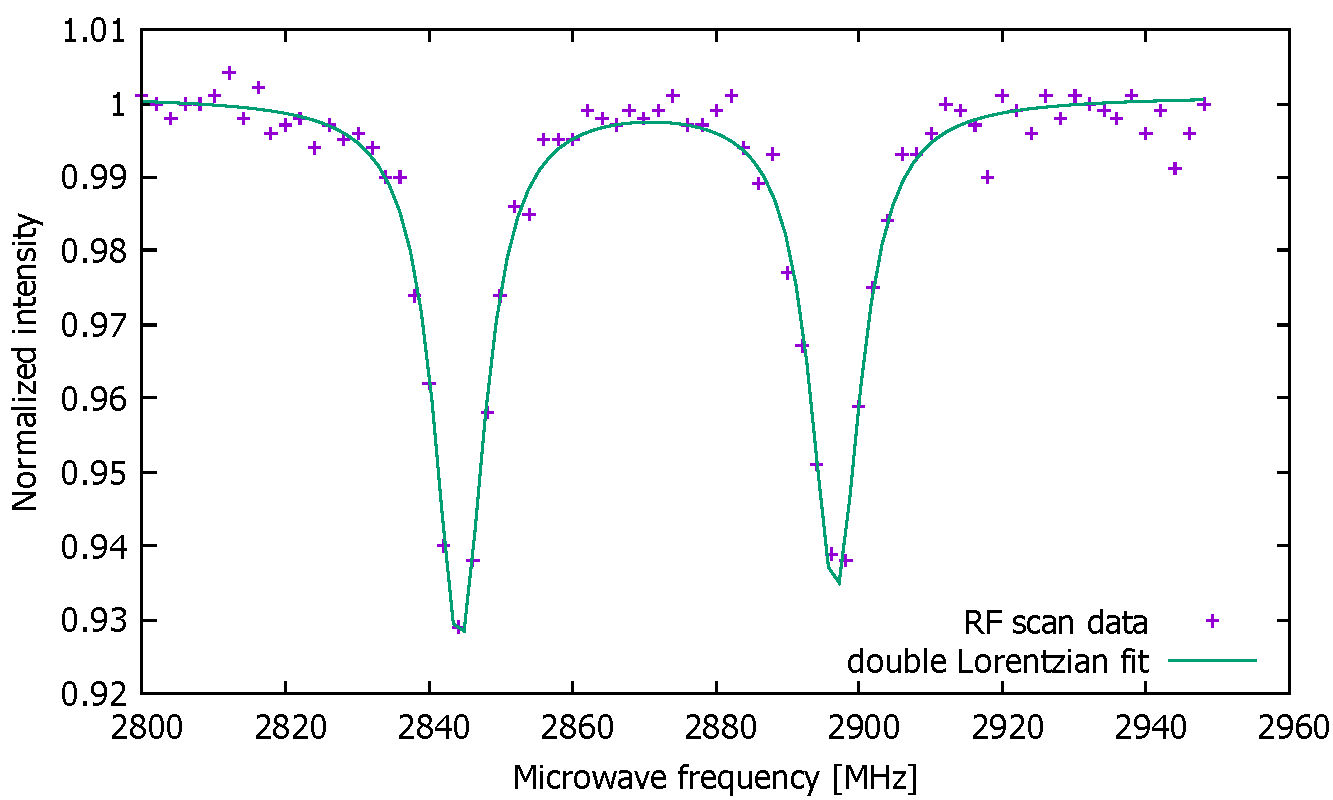
\includegraphics[scale=0.6]{rfbulk.pdf} 
\caption{RF scan on the spin bath of the Bulk diamond, revealing two resonances separated by about 50 MHz.}
\label{rfb}
\end{figure}
For the decoupling sequences, the first resonant frequency was chosen.
\\
The conduct of Rabi oscillations (figure \ref{br}) reveals a very high $\pi$ pulse length of about $\unit[372]{ns}$, which is 4 times as long as for the nanodiamond measurement.\\
\begin{figure}[H]
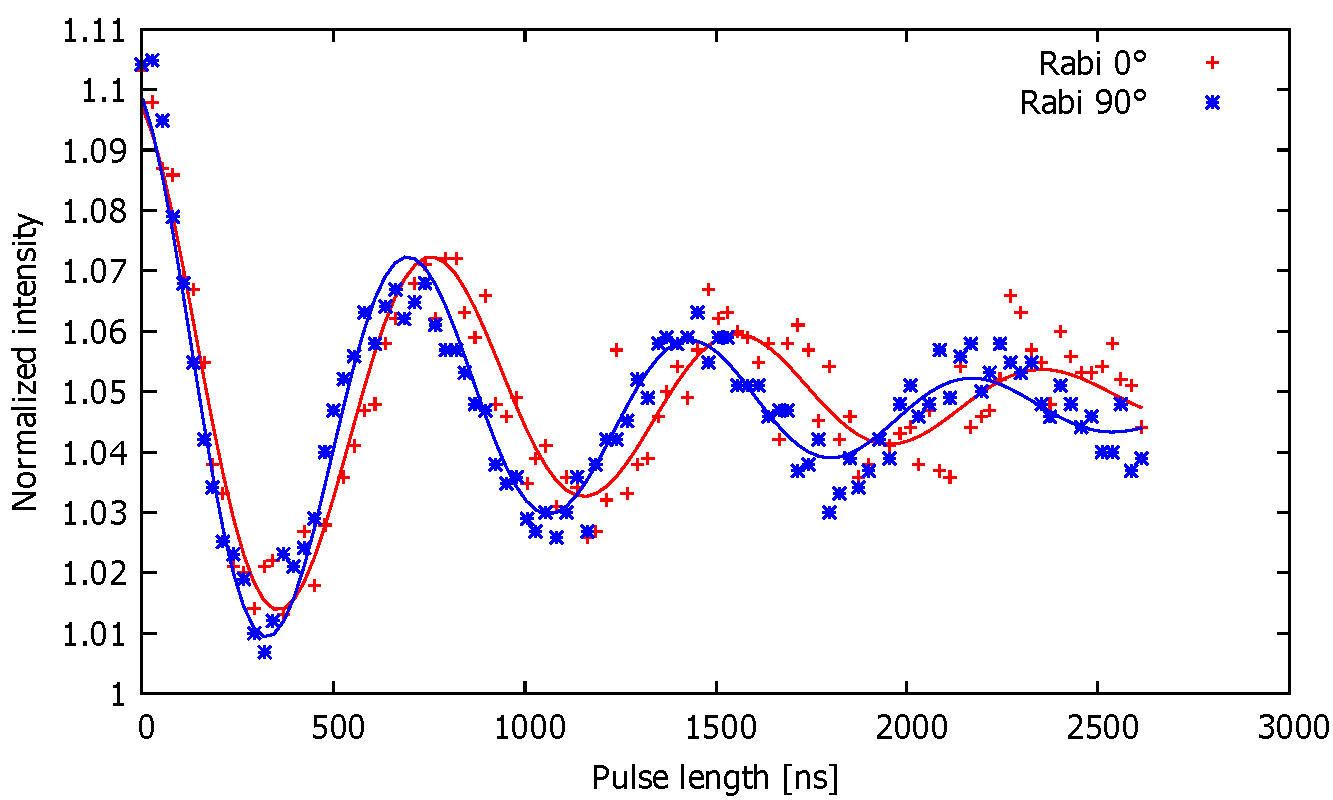
\includegraphics[scale=0.6]{bulkrabi.pdf} 
\caption{Rabi oscillations with both phases on the spin bath.}
\label{br}
\end{figure} 
\subsubsection{Decoupling sequences}  
The corresponding Hahn Echo (figure \ref{bh}) exhibits a faster decay if compared with all of the NVs in nanodiamonds precedently observed.
As the ensemble of NVs is expected to be in an incoherent mixture between the $m_s=0$ and $m_s=-1$ states after the Hahn echo decay, another mechanism seems to drive the system back to $m_s=0$. Indeed, the low contrast allows us to observe an unexpected slow increase in the normalized intensity for times higher than 500 ns. This has been found to be related to small drifts in the effective laser power used in the sequence, likely due to electronic effects in the Acousto Optic Modulator used to pulse the laser. 
%This aspect will be discussed further during the evaluation of the decoupling sequences. \\
\begin{figure}[H]
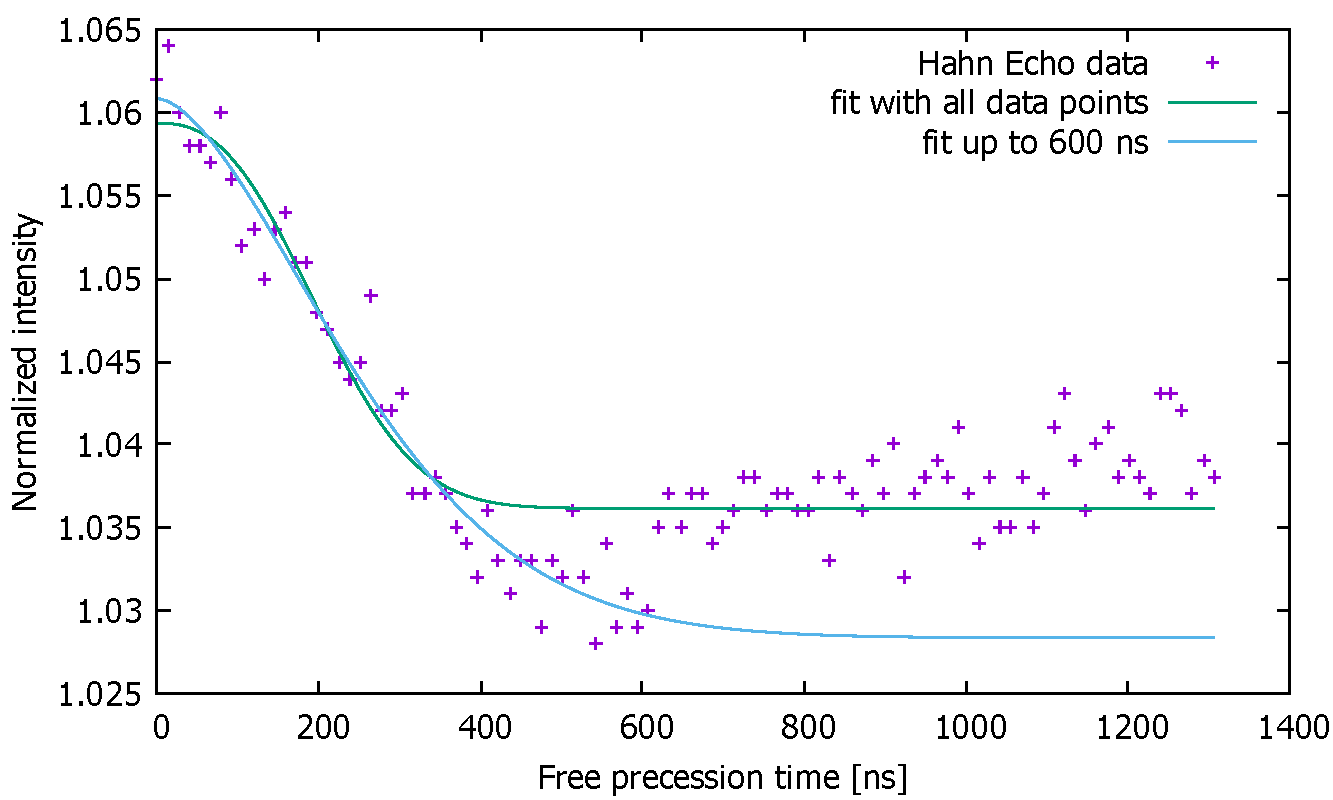
\includegraphics[scale=0.6]{bulkhahn.pdf} 
\caption{Hahn Echo for the Bulk diamond. After an initial decay, the intensity increases again, suggesting an additional effect that drives the spin back to the bright state. For this reason, two different fits have been made: the first fit included all data points, the second one only the points which describe the actual decay that occurs for relaxation times below 600 ns.}
\label{bh}
\end{figure}
The ordinary fit that factors in all data points results in a relaxation time of $T_2=\unit[(235\pm 13)]{ns}$. By observing that the increase of intensity is independent of the relaxation caused by the spin bath, an alternative fit has been made, excluding relaxation times of more than 600 ns. From that, one gets $T_2=\unit[(302\pm 25)]{ns}$. For the investigation of coherence time improvement through dynamical decoupling, the $T_2$ time acquired from the adjusted fit will be considered the actual relaxation time.

In order to compensate for the AOM effects, a reference measurement was done in addition to every scan. So, after the performance of dynamical decoupling, the same sequence was conducted with an off-set microwave, meaning a Rf frequency 100 MHz below resonance. As external driving and dynamical decoupling both cause an increase of intensity, the scans looked very similar. This is why also decoupling sequences with a finite $\nicefrac{3\pi}{2}$ were implemented, because the effects of driving and dynamical decoupling would now compensate each other. An example of all 3 types of scans is shown in figure \ref{cr}.\\
\begin{figure}[H]
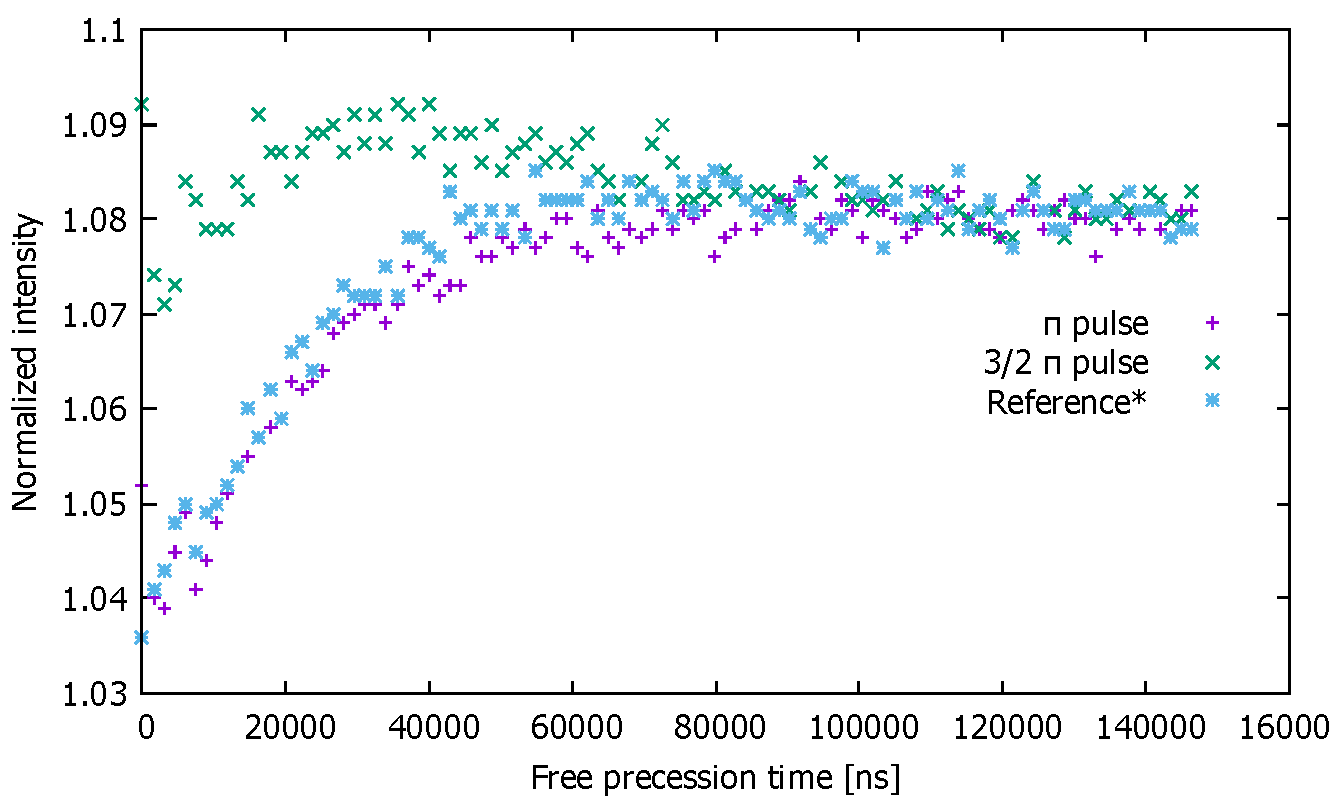
\includegraphics[scale=0.6]{cref.pdf} 
\caption{Examination of the driving for CPMG-16. The reference dataset was shifted by a constant for better comparison. The conventional measurement and the reference look almost similar; the sequence with a finite $3\pi/2$ pulse differs from the other two.}
\label{cr}
\end{figure}
Getting meaningful data required to subtract the driving effect from the decoupling. For this, there were 3 options: one could remove the background from either the conventional or the $3\pi/2$ measurement, or one could directly combine both decoupling measurements. Attempting to gain the highest possible contrast, latter has been done. Analogous to the visibility in interferometric experiments, an effective contrast has been introduced in the form of:
\begin{equation}
I=\frac{I(3\pi/2)-I(\pi)}{I(3\pi/2)+I(\pi)}
\end{equation}
for the decoupling sequences. 
\paragraph{CPMG}\mbox{}\\
Due to the low contrast, the decoupling sequences were only conducted up to a length of 32 pulses. \\
\begin{figure}[H]
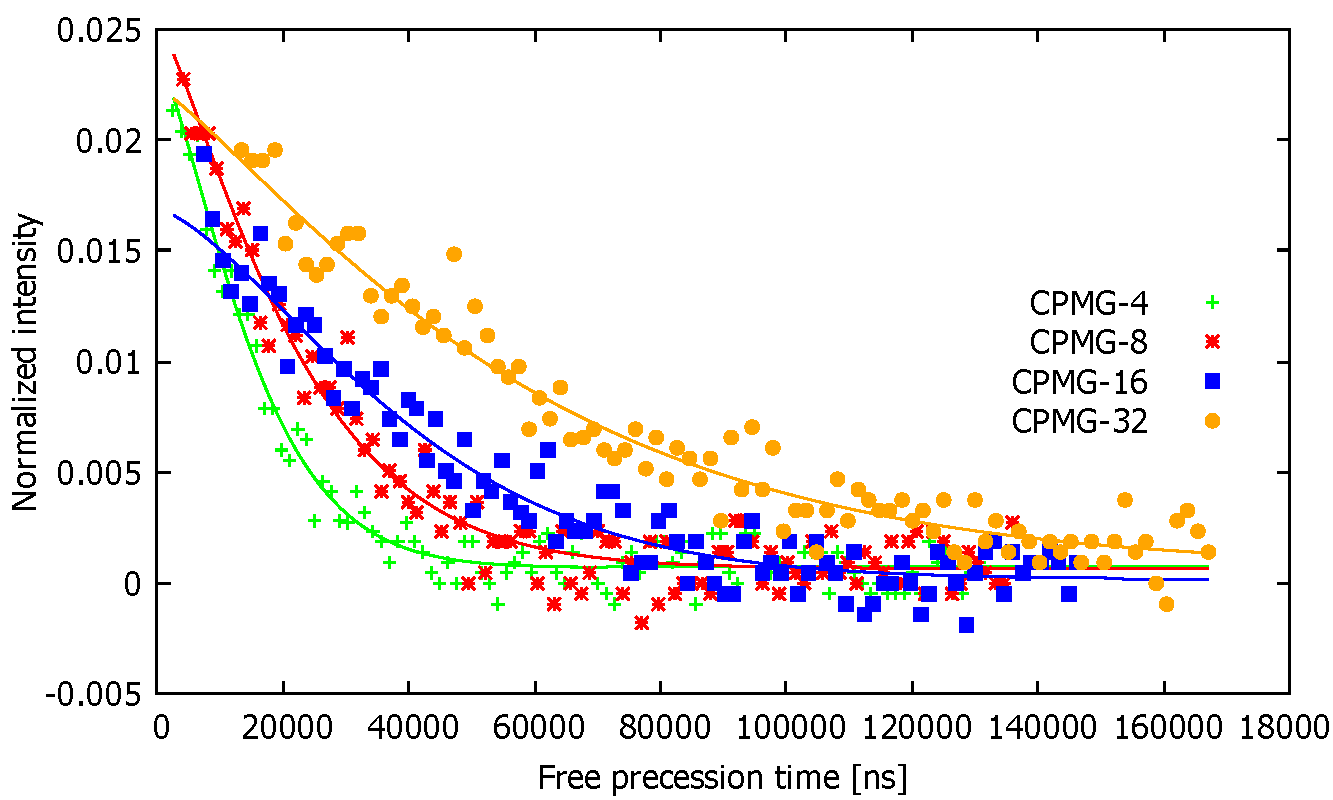
\includegraphics[scale=0.6]{cpbulk.pdf} 
\caption{CPMG on the Bulk diamond for different numbers of pulses. A continuous increase of the coherence time can be observed.}
\label{cb}
\end{figure}
The plot (figure \ref{cb}) shows that the coherence time gradually increases with the number of pulses. This gets also verified by the fit parameters (table \ref{c4b}). While $\alpha$ still shows no consistent behaviour, the coherence time rises up to 60 $\mu$s which corresponds to almost 200 times $T_2$.\\
\begin{table}[H]
\centering
\caption{CPMG fit parameters for different numbers of $\pi$ pulses}
\label{c4b}
\begin{tabular}{l|lll}
number of pulses &   exponent $\alpha$   & coherence time {[}ns{]}   & $t_0$/$T_2$   \\\hline
4                &   1.44$\pm$ 0.10      & 17200$\pm$ 700                      & 57 \\
8                &   1.22$\pm$ 0.10      & 23100$\pm$ 1100                    & 77\\
16               &   1.54$\pm$ 0.15      & 44500$\pm$ 1900                     & 148 \\
32               &   1.17$\pm$ 0.11      & 59500$\pm$ 3100                     & 197
\end{tabular}
\end{table}
Compared to the nanodiamond, the improvement of coherence time has increased by almost an order of magnitude.
\paragraph{XY}\mbox{}\\
Also the XY sequence was only conducted up to 32 pulses. The plot (figure \ref{xb}) makes clear that all XY sequences on the spin bath give the same result. In conclusion, XY-8 already achieves the maximum coherence time possible with an XY pulse sequence for the spin bath. The fit data (table \ref{x4b}) support this observation: sequences with more pulses don't accomplish a distinct improvement of the $T_2$ time with respect to XY-8.
\begin{figure}[H]
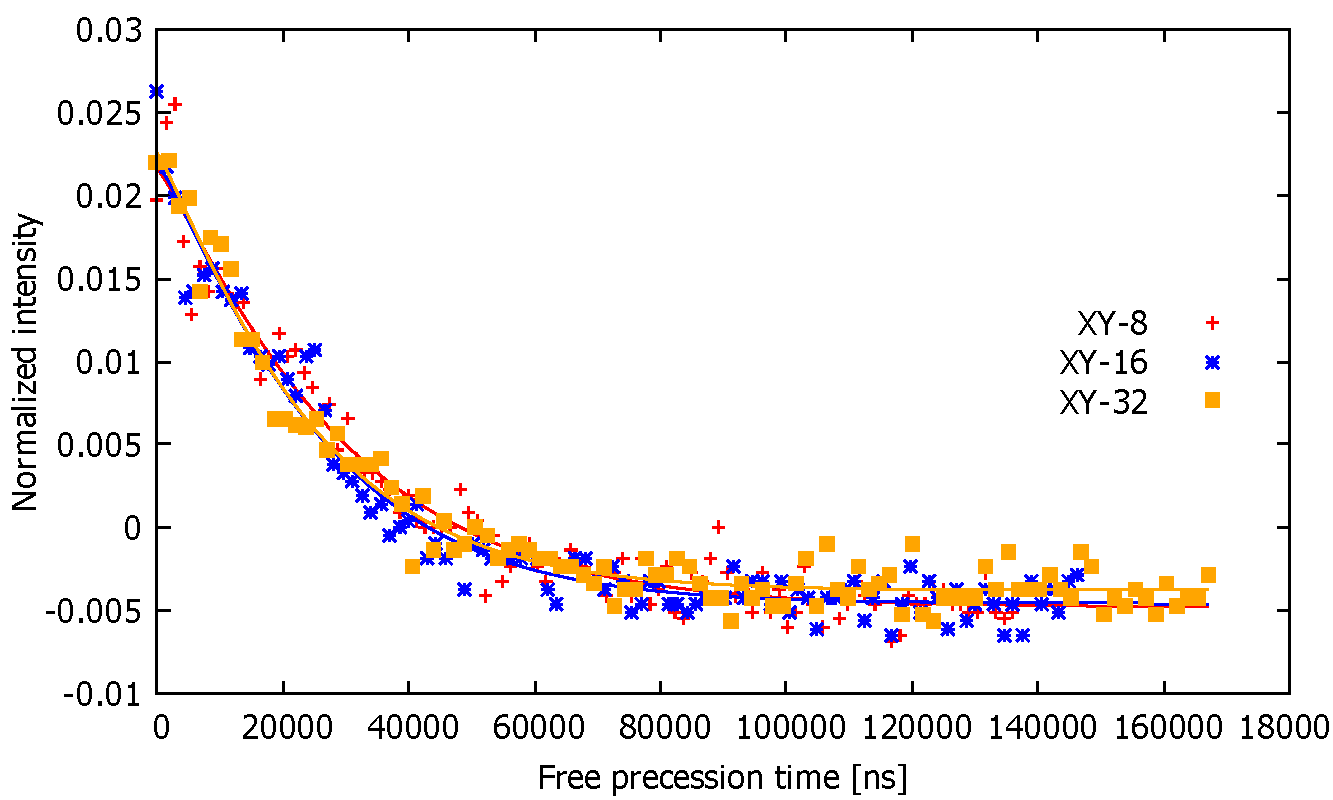
\includegraphics[scale=0.6]{xybulk.pdf} 
\caption{XY on the Bulk diamond for different numbers of pulses. All scans give almost similar results.}
\label{xb}
\end{figure}
\begin{table}[H]
\centering
\caption{XY fit parameters for different numbers of $\pi$ pulses}
\label{x4b}
\begin{tabular}{l|lll}
number of pulses &   exponent $\alpha$   & coherence time {[}ns{]}   & $t_0$/$T_2$   \\\hline
8                &   1.02$\pm$ 0.10      & 28500$\pm$ 1700                    & 94\\
16               &   1.46$\pm$ 0.12      & 29600$\pm$ 1200                     & 98 \\
32               &   1.11$\pm$ 0.10      & 24500$\pm$ 1400                     & 81
\end{tabular}
\end{table}

\paragraph{Comparison of XY and CPMG}\mbox{}\\
As shown before, CPMG gradually enhances the coherence time with an increasing number of pulses whereas XY-8 already achieves the highest coherence time for XY sequences. Consequently, if 8 pulses are applied, the XY gives better results than CPMG. However, when more pulses are applied, CPMG outperforms XY and reaches up to twice the coherence time. \\
Therefore, CPMG also realizes a better decoupling of the NV spin from the spin bath of a Bulk diamond.
\begin{figure}[H]
\centering
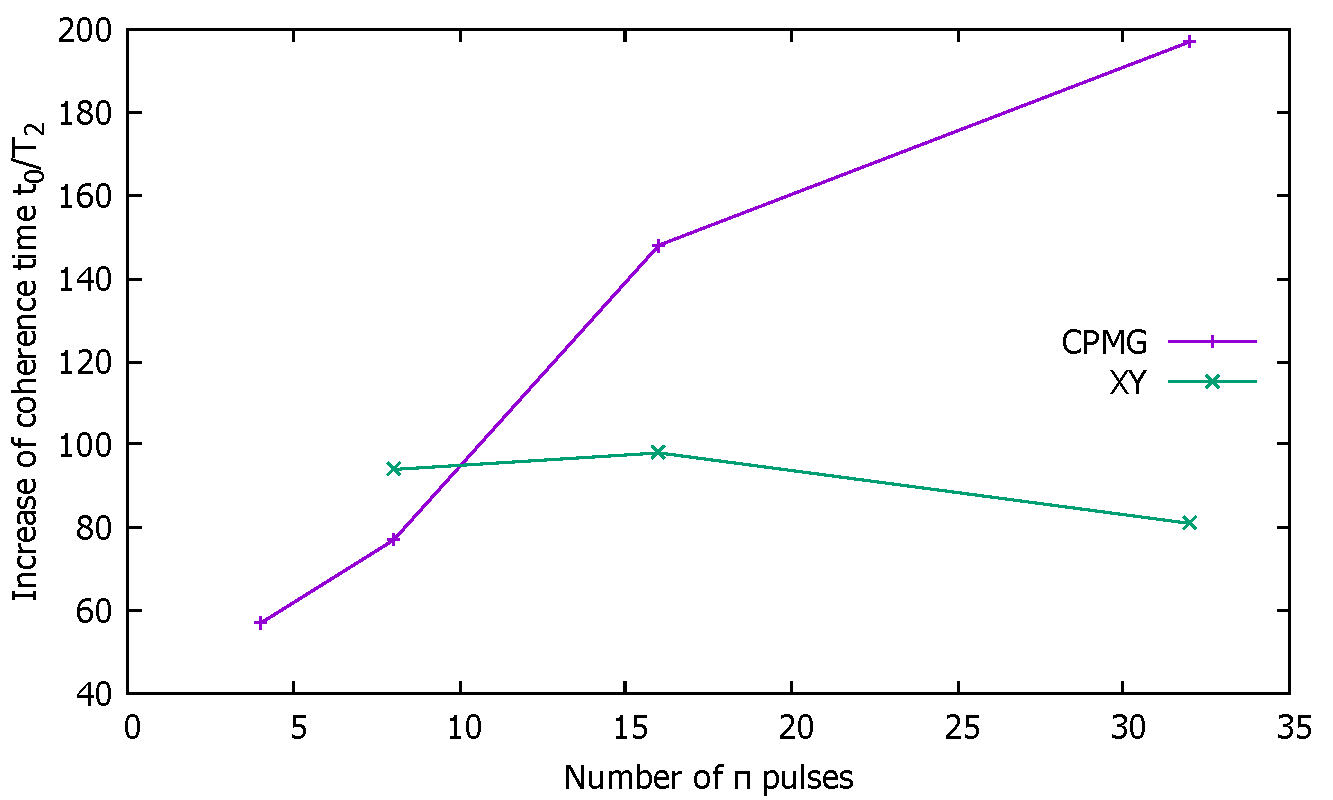
\includegraphics[scale=0.6]{bulkcx2.pdf} 
\caption{Comparison of XY and CPMG sequences on the spin bath: while the coherence time stagnates for XY, it continuously increases under CPMG.}
\label{xcb}
\end{figure}
\subsubsection{Spectral decomposition}
Also the Measurements on the Bulk diamond were further evaluated. As before, just the CPMG data were examined.\\
Similarly to the nanodiamond, also the computations with the data from the Bulk diamond reveal a dependency between the two variables.
\begin{figure}[h!]\label{HB} 
    \subfigure[]{\includegraphics[width=0.55\textwidth]{hahnbulk.pdf}} 
    \subfigure[]{\includegraphics[width=0.49\textwidth]{bdc32.pdf}} 
    \caption{Determination of the parameters $\Delta$ and $\tau_c$ from the measurements on the Bulk: figure (a) shows a calculation for the Hahn Echo over multiple orders of magnitude, figure (b) presents the analysis of CPMG-32. In blue regions, the deviation reaches a minimum, for yellow it is highest. The red dot represents the point with the minimal deviation from the data.}
\end{figure}
\newpage
Again, after doing all calculations, one gets for the different spectral distributions:
%\begin{figure}[H]\label{sb} 
%    \subfigure[]{\includegraphics[width=0.49\textwidth]{bd12.pdf}} 
%    \subfigure[]{\includegraphics[width=0.49\textwidth]{bd22.pdf}} 
%    \caption{Spectral density functions for different CPMG measurements and the Hahn Echo. From the computations, one gets $\unit[240]{ns}\leq\tau_c\leq\unit[700]{ns}$ and $\unit[1.7]{MHz}\leq\Delta\leq\unit[2.5]{MHz}$ for CPMG and for the Hahn Echo $\tau_c=\unit[65]{ns}$ and $\Delta=\unit[94]{MHz}$.}
%\end{figure}
\begin{figure}[H]
\centering
\includegraphics[scale=0.6]{bd12.pdf} 
\caption{Spectral density functions for different CPMG measurements and the Hahn Echo. From the computations, one gets $\unit[240]{ns}\leq\tau_c\leq\unit[700]{ns}$ and $\unit[1.7]{MHz}\leq\Delta\leq\unit[2.5]{MHz}$ for CPMG and for the Hahn Echo $\tau_c=\unit[65]{ns}$ and $\Delta=\unit[94]{MHz}$.}
\label{sb}
\end{figure}
The parameters extracted from CPMG agree well with similar measurements, where $\unit[0]{MHz}\leq\Delta\leq\unit[10]{MHz}$ and $\unit[1]{\mu s}\leq\tau_c\leq\unit[15]{\mu s}$. Only $\tau_c$ is about one order of magnitude smaller, indicating a higher N density for the sample used in our setup.\\
As observed for the nanodiamond, the Hahn Echo spectrum amplitude is more than one order of magnitude larger, thus showing a consistent behaviour.
\subsection{Comparison of nanodiamond and Bulk diamond}
For both the single NV electron spins in the nanodiamond and the NV spin ensemble of the Bulk diamond, CPMG performed better than XY. While having prolonged the coherence time of a single spin by an order of magnitude, the $T_2$ time of the NV spin bath could be improved by more than two orders of magnitude. However, the achieved maximum coherence time was in both cases in the range of 60 $\mu s$, so this criterion favours neither nanodiamond nor the Bulk. Despite the surface effects, single NVs in nanodiamond may perform better due to higher contrast with respect to large NV ensembles in the Bulk and thus be more suitable for magnetometry measurements because of a better sensitivity. The sensitivity can be calculated according to \cite{diss}:
\begin{equation}
\eta=\frac{\pi\hbar}{2 g\mu_B C\sqrt{N\cdot T_2}}
\end{equation}
where $C$ is the contrast, $N$ is the number of NV centers contributing to the signal and $T_2$ is the maximum achieved coherence time. This yields for the nanodiamond a sensitivity of $\eta_{N}\approx \unit[10]{nT/\sqrt{Hz}}$ and for the bulk sample $\eta_{BD}=\unit[(6-18)]{nT/\sqrt{Hz}}$ for 10 to 100 estimated contributing NV centers.
\newpage
\section{Conclusion and Outlook}
During the work for this thesis, different dynamical decoupling protocols have been implemented. It was demonstrated that all of these protocols were able to prolong the NV electron spin coherence time in Bulk diamond and nanodiamond. In particular, the CPMG sequences could enhance the NV electron spin coherence time by a factor of up to 50 in the nanodiamond and 200 in the Bulk diamond, leading to coherence times of $\unit[60]{\mu s}$. In connection with that, it was found that single-axis control via CPMG outperforms two-axis decoupling through XY-sequences for both the nanodiamond and the Bulk diamond. Additionally, it was observed that the same decoupling sequences achieved different coherence time improvements on different nanodiamonds.
\\
Furthermore, the spectral density of the spin bath could be obtained, with good agreement to other results for the Bulk diamond. In order to find the mechanisms causing dephasing of NV electron spins, further research on this subject is crucial.
\\
For the implementation of sequences with time-dependent pulse spacings in the form of UDD, it was shown that the arrangement of the pulse centers according to the theoretical model leads to a higher coherence time. However, because of the finite resolution of the BPG, the UDD protocol was executed in a non-optimal way on this setup. But the finite BPG resolution did not only affect the UDD sequence. In fact, for the execution of any sequence, the $\pi$ pulse length is rounded to multiples of 6.6 ns and thereby gets faulty. These pulse errors accumulate\cite{pea} and set a limit on the number of pulses that can be applied. In this context, also the finite length of the pulses distorts the measurements, regarding that all pulse sequences were derived under the assumption of perfect $\delta$ pulses. Thus, especially for short free precession times, the pulses have a comparable duration. Unfortunately, increasing the MW power and thereby shortening the pulse length also requires a more precise BPG in order to avoid additional pulse errors. In addition to that, the Rabi oscillations 
showed discrepancies of up to 10\% between the two MW phases regarding the $\pi$ pulse length, which may also be the reason for lower coherence times with XY. Finally, the likely AOM-related drift of the NV spin state for long precession times needs to be further investigated.\\
In the future, the performance of sequences with more pulses should be examined with the aim of exploring the limitations and their reasons. With a better time and phase control in the form of a more precise BPG, UDD will be further investigated and other two-axis decoupling protocols\cite{qdd} can be tested. 



\bibliography{quellen}
\bibliographystyle{ieeetr}
\section*{Selbst\"andigkeitserkl\"arung}


Ich erkl\"are hiermit, dass ich die vorliegende Arbeit selbst\"andig verfasst und 
noch nicht f\"ur andere Pr\"ufungen eingereicht habe. S\"amtliche Quellen 
einschlie\ss lich Internetquellen, die unver\"andert oder abgewandelt wiedergegeben 
werden, insbesondere Quellen f\"ur Texte, Grafiken, Tabellen und Bilder, sind als 
solche kenntlich gemacht. Mir ist bekannt, dass bei Verst\"o\ss en gegen diese 
Grunds\"atze ein Verfahren wegen T\"auschungsversuchs bzw. T\"auschung eingeleitet 
wird.\\[3cm]
%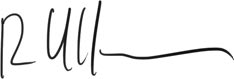
\includegraphics{unterschrift_richard}\\ 
Berlin, \dcdatesubmitted
\end{document}

